% Options for packages loaded elsewhere
\PassOptionsToPackage{unicode}{hyperref}
\PassOptionsToPackage{hyphens}{url}
\PassOptionsToPackage{dvipsnames,svgnames*,x11names*}{xcolor}
%
\documentclass[
  10pt,
]{article}
\usepackage{amsmath,amssymb}
\usepackage{lmodern}
\usepackage{ifxetex,ifluatex}
\ifnum 0\ifxetex 1\fi\ifluatex 1\fi=0 % if pdftex
  \usepackage[T1]{fontenc}
  \usepackage[utf8]{inputenc}
  \usepackage{textcomp} % provide euro and other symbols
\else % if luatex or xetex
  \usepackage{unicode-math}
  \defaultfontfeatures{Scale=MatchLowercase}
  \defaultfontfeatures[\rmfamily]{Ligatures=TeX,Scale=1}
\fi
% Use upquote if available, for straight quotes in verbatim environments
\IfFileExists{upquote.sty}{\usepackage{upquote}}{}
\IfFileExists{microtype.sty}{% use microtype if available
  \usepackage[]{microtype}
  \UseMicrotypeSet[protrusion]{basicmath} % disable protrusion for tt fonts
}{}
\makeatletter
\@ifundefined{KOMAClassName}{% if non-KOMA class
  \IfFileExists{parskip.sty}{%
    \usepackage{parskip}
  }{% else
    \setlength{\parindent}{0pt}
    \setlength{\parskip}{6pt plus 2pt minus 1pt}}
}{% if KOMA class
  \KOMAoptions{parskip=half}}
\makeatother
\usepackage{xcolor}
\IfFileExists{xurl.sty}{\usepackage{xurl}}{} % add URL line breaks if available
\IfFileExists{bookmark.sty}{\usepackage{bookmark}}{\usepackage{hyperref}}
\hypersetup{
  colorlinks=true,
  linkcolor=Maroon,
  filecolor=Maroon,
  citecolor=Blue,
  urlcolor=blue,
  pdfcreator={LaTeX via pandoc}}
\urlstyle{same} % disable monospaced font for URLs
\usepackage[left=2cm, right=2cm, top=2cm, bottom=3cm, footskip =
.5cm]{geometry}
\usepackage{graphicx}
\makeatletter
\def\maxwidth{\ifdim\Gin@nat@width>\linewidth\linewidth\else\Gin@nat@width\fi}
\def\maxheight{\ifdim\Gin@nat@height>\textheight\textheight\else\Gin@nat@height\fi}
\makeatother
% Scale images if necessary, so that they will not overflow the page
% margins by default, and it is still possible to overwrite the defaults
% using explicit options in \includegraphics[width, height, ...]{}
\setkeys{Gin}{width=\maxwidth,height=\maxheight,keepaspectratio}
% Set default figure placement to htbp
\makeatletter
\def\fps@figure{htbp}
\makeatother
\setlength{\emergencystretch}{3em} % prevent overfull lines
\providecommand{\tightlist}{%
  \setlength{\itemsep}{0pt}\setlength{\parskip}{0pt}}
\setcounter{secnumdepth}{-\maxdimen} % remove section numbering
% Set up the fonts
\usepackage[urw-palatino]{mathdesign}
\usepackage[T1]{fontenc}


% Set the language for 508
\hypersetup{
  pdftitle = {title},
  pdflang = en-US}

% Add accessibility support from http://www.richschwinn.com/accessibility
\RequirePackage{accsupp}
\RequirePackage{pdfcomment}
\newcommand{\AccTool}[2]{\BeginAccSupp{method=pdfstringdef,unicode,Alt={{#1}}}\pdftooltip{{#2}}{{#1}}\EndAccSupp{}}


% Set up the headers and footers
\usepackage{graphicx}
\usepackage{fancyhdr}
\usepackage{ifthen}
%\usepackage{everypage-1x}
\usepackage{float}
%\usepackage{subfig}
%\usepackage{subcaption}

% Avoid struggling over figure and table float in Rmarkdown
\let\origfigure\figure
\let\endorigfigure\endfigure
\renewenvironment{figure}[1][2] {
    \expandafter\origfigure\expandafter[H]
} {
    \endorigfigure
}

\let\origtable\table
\let\endorigtable\endtable
\renewenvironment{table}[1][2] {
    \expandafter\origtable\expandafter[H]
} {
    \endorigtable
}

% First page has the large title and NOAA logo
\pagestyle{fancy}
\fancyhf{}
\setlength\headheight{40pt}
\fancyheadoffset[L]{0.5cm}
\cfoot{\thepage}

\fancyheadinit{%
   \ifthenelse{\value{page}=4}%
      {\fancyhead[R]{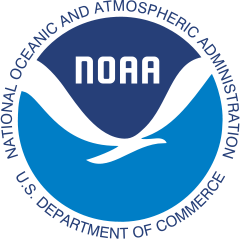
\includegraphics[width=40pt]{images/NOAA_logo.png} \\ \textsf{\emph{March 17, 2022}}}
       \fancyhead[L]{\textsf{\LARGE State of the Ecosystem 2022: Mid-Atlantic}}
      }%
      {\fancyhead[R]{}
       \fancyhead[L]{\textsf{\emph{State of the Ecosystem 2022: Mid-Atlantic}}}
      }
}



\renewcommand{\headrulewidth}{0.4pt}
\renewcommand{\footrulewidth}{0pt}

% Make caption fonts a bit smaller
\usepackage[font={small}]{caption}


% Change section labels to san serif
\usepackage{sectsty}
\allsectionsfont{\normalfont\sffamily\bfseries}
\usepackage{booktabs}
\usepackage{longtable}
\usepackage{array}
\usepackage{multirow}
\usepackage{wrapfig}
\usepackage{float}
\usepackage{colortbl}
\usepackage{pdflscape}
\usepackage{tabu}
\usepackage{threeparttable}
\usepackage{threeparttablex}
\usepackage[normalem]{ulem}
\usepackage{makecell}
\usepackage{xcolor}
\ifluatex
  \usepackage{selnolig}  % disable illegal ligatures
\fi
\newlength{\cslhangindent}
\setlength{\cslhangindent}{1.5em}
\newlength{\csllabelwidth}
\setlength{\csllabelwidth}{3em}
\newenvironment{CSLReferences}[2] % #1 hanging-ident, #2 entry spacing
 {% don't indent paragraphs
  \setlength{\parindent}{0pt}
  % turn on hanging indent if param 1 is 1
  \ifodd #1 \everypar{\setlength{\hangindent}{\cslhangindent}}\ignorespaces\fi
  % set entry spacing
  \ifnum #2 > 0
  \setlength{\parskip}{#2\baselineskip}
  \fi
 }%
 {}
\usepackage{calc}
\newcommand{\CSLBlock}[1]{#1\hfill\break}
\newcommand{\CSLLeftMargin}[1]{\parbox[t]{\csllabelwidth}{#1}}
\newcommand{\CSLRightInline}[1]{\parbox[t]{\linewidth - \csllabelwidth}{#1}\break}
\newcommand{\CSLIndent}[1]{\hspace{\cslhangindent}#1}

\author{}
\date{\vspace{-2.5em}}

\begin{document}

\setcounter{page}{4}
\thispagestyle{fancy}

\hypertarget{introduction}{%
\section{Introduction}\label{introduction}}

\hypertarget{about-this-report}{%
\subsection{About This Report}\label{about-this-report}}

This report is for the Mid-Atlantic Fishery Management Council (MAFMC).
The purpose of this report is to synthesize ecosystem information to
allow the MAFMC to better meet fishery management objectives, and to
update the MAFMC's Ecosystem Approach to Fishery Management (EAFM) risk
assessment. The major messages of the report are synthesized on pages 1
and 2, and synthesis themes are illustrated on page 3. The information
in this report is organized into two sections;
\protect\hyperlink{performance-relative-to-fishery-management-objectives}{performance
measured against ecosystem-level management objectives} (Table
\ref{tab:management-objectives}), and potential
\protect\hyperlink{risks-to-meeting-fishery-management-objectives}{risks
to meeting fishery management objectives}
(\protect\hyperlink{climate-and-ecosystem-productivity}{climate change}
and \protect\hyperlink{other-ocean-uses-offshore-wind}{other ocean
uses}).

\hypertarget{report-structure}{%
\subsection{Report structure}\label{report-structure}}

The two main sections contain subsections for each management objective
or potential risk. Within each subsection, we first review indicator
trends, and the status of the most recent data year relative to a
threshold (if available) or relative to the long-term average. Second,
we synthesize results of other indicators and information to outline
potential implications for management (i.e., connecting indicator(s)
status to management and why an indicator(s) is important). For example,
if there are multiple drivers related to an indicator trend, which
drivers may be more or less supported by current information, and which,
if any, can be affected by management action(s)? Similarly, which risk
indicators warrant continued monitoring to evaluate whether regime
shifts or ecosystem reorganization are likely? We emphasize that these
implications are intended to represent testable hypotheses at present,
rather than ``answers,'' because the science behind these indicators and
syntheses continues to develop.

A glossary of terms\footnote{\url{https://noaa-edab.github.io/tech-doc/glossary.html}},
detailed technical methods documentation\footnote{\url{https://NOAA-EDAB.github.io/tech-doc}},
and indicator data\footnote{\url{https://github.com/NOAA-EDAB/ecodata}}
are available online. The details of standard figure formatting (Fig.
\ref{fig:docformat}a), categorization of fish and invertebrate species
into feeding guilds (Table \ref{tab:species-groupings}), and definitions
of ecological production units (EPUs, including the Mid-Atlantic Bight,
MAB; Fig. \ref{fig:docformat}b) are provided at the end of the document.

\begin{table}[!h]

\caption{\label{tab:management-objectives}Ecosystem-scale fishery management objectives in the Mid-Atlantic Bight}
\centering
\begin{tabular}[t]{ll}
\toprule
\textbf{Objective Categories} & \textbf{Indicators reported}\\
\midrule
\addlinespace[0.3em]
\multicolumn{2}{l}{\textbf{Provisioning and Cultural Services}}\\
\hspace{1em}Seafood Production & Landings; commercial total and by feeding guild; recreational harvest\\
\hspace{1em}Profits & Revenue decomposed to price and volume\\
\hspace{1em}Recreation & Angler trips; recreational fleet diversity\\
\hspace{1em}Stability & Diversity indices (fishery and ecosystem)\\
\hspace{1em}Social \& Cultural & Community engagement/reliance and environmental justice status\\
\hspace{1em}Protected Species & Bycatch; population (adult and juvenile) numbers, mortalities\\
\addlinespace[0.3em]
\multicolumn{2}{l}{\textbf{Supporting and Regulating Services}}\\
\hspace{1em}Biomass & Biomass or abundance by feeding guild from surveys\\
\hspace{1em}Productivity & Condition and recruitment of managed species, primary productivity\\
\hspace{1em}Trophic structure & Relative biomass of feeding guilds, zooplankton\\
\hspace{1em}Habitat & Estuarine and offshore habitat conditions\\
\bottomrule
\end{tabular}
\end{table}

\hypertarget{performance-relative-to-fishery-management-objectives}{%
\section{Performance Relative to Fishery Management
Objectives}\label{performance-relative-to-fishery-management-objectives}}

In this section, we examine indicators related to broad, ecosystem-level
fishery management objectives. We also provide hypotheses on the
implications of these trends---\emph{why} we are seeing them, what's
driving them, and potential or observed regime shifts or changes in
ecosystem structure. Identifying multiple drivers, regime shifts, and
potential changes to ecosystem structure, as well as identifying the
most vulnerable resources, can help managers determine whether we can do
anything differently to meet objectives and how to prioritize for
upcoming issues/risks.

\emph{Special note on data availability for the 2022 report}

The Catch Accounting and Monitoring System (CAMS) that will be used to
provide commercial landings and discard information at the Ecological
Production Unit (EPU) scale is under development. As of February 2022,
our standard indicators relying on EPU scale landings data cannot be
calculated for 2020 (commercial seafood production, commercial profits,
ecosystem overfishing). We provide information based on coastwide
commercial landings information available at this time in
{[}\protect\hyperlink{ref-thunberg_northeast_2021}{1}{]}\footnote{\url{https://spo.nmfs.noaa.gov/sites/default/files/TM221.pdf}},
and will calculate our standard indicators at EPU scales with
disaggregated 2020 commercial landings data when they are available.

\hypertarget{seafood-production}{%
\subsection{Seafood Production}\label{seafood-production}}

\hypertarget{indicators-landings-commercial-and-recreational}{%
\subsubsection{Indicators: Landings; commercial and
recreational}\label{indicators-landings-commercial-and-recreational}}

Total commercial landings (black) within the Mid-Atlantic are not yet
available for 2020; Figure \ref{fig:total-landings} includes data only
through 2019. However, we do not anticipate the long-term declining
trend in landings to change.

Coastwide landings at the Federal fishery management plan (FMP) level
were mixed in 2020 when compared to recent years
{[}\protect\hyperlink{ref-thunberg_northeast_2021}{1}{]}. Landings of
monkfish and of combined surfclam and ocean quahog declined in 2020,
while landings of combined summer flounder, scup, and black sea bass
increased, and landings of combined squid species increased in 2020.

\begin{figure}

{\centering \includegraphics{docs/images/total-landings-1} 

}

\caption{Total commercial seafood landings through 2019 (black) and Mid-Atlantic managed seafood landings (red).}\label{fig:total-landings}
\end{figure}

Total recreational harvest (retained fish presumed to be eaten) is down
in the MAB (Fig. \ref{fig:rec-landings}). Although harvest has increased
from a historic low in 2018, it is still below the average value for the
series.

\begin{figure}

{\centering \includegraphics{docs/images/rec-landings-1} 

}

\caption{Total recreational seafood harvest (millions of pounds) in the Mid-Atlantic region.}\label{fig:rec-landings}
\end{figure}

Recreational shark landings show an increase in pelagic sharks over the
past decade, with a sharp decrease in 2018 - 2019 persisting through
2021 (Fig \ref{fig:rec_hms}). This is likely influenced by regulatory
changes implemented in 2018 intended to rebuild shortfin mako stocks. In
2021 the International Commission for the Conservation of Atlantic Tunas
(ICCAT) finalized recommendations for a two-year retention ban (ICCAT
Rec.21-09), which will also affect total overall landings of pelagic
sharks in coming years.

\begin{figure}

{\centering \includegraphics{docs/images/rec_hms-1} 

}

\caption{Recreational shark landings from Marine Recreational Information Program.}\label{fig:rec_hms}
\end{figure}

Aquaculture production is not yet included in total seafood landings,
but we are working toward including it in future reports. Available
aquaculture production of oysters for a subset of Mid-Atlantic states is
trending upward.\footnote{\url{https://noaa-edab.github.io/ecodata/human_dimensions_MAB\#Commercial};
  ``Oyster Aquaculture'' tab}

\hypertarget{implications}{%
\subsubsection{Implications}\label{implications}}

Declining commercial and recreational landings can be driven by many
interacting factors, including combinations of ecosystem and stock
production, management actions, market conditions (including COVID-19
disruptions), and environmental change. While we cannot evaluate all
possible drivers at present, here we evaluate the extent to which stock
status and system biomass trends may play a role.

\hypertarget{stock-status-and-catch-limits}{%
\paragraph{Stock Status and Catch
Limits}\label{stock-status-and-catch-limits}}

Single species management objectives (1. maintaining biomass above
minimum thresholds and 2. maintaining fishing mortality below
overfishing limits) are being met for all but two MAFMC managed species,
though the status of six stocks is unknown (Fig.
\ref{fig:stock-status}).

\begin{figure}

{\centering \includegraphics{docs/images/stock-status-1} 

}

\caption{Summary of single species status for MAFMC and jointly federally managed stocks (Spiny dogfish and both Goosefish). The dotted verticxal line is the target bioomass reference point of Bmsy. The dashed lines are the management trehsolds of one half Bmsy (vertical) or Fmsy (horizontal). Stocks in green are below the biomass threshold (overfished), stocks in orange are above the biomass threshold but below the biomass target, and stocks in purple are above the biomass target. Only one stock, Atlantic mackerel, has fishing mortality above the limit (subject to overfishing).}\label{fig:stock-status}
\end{figure}

Stock status affects catch limits established by the Council, which in
turn may affect landings trends. Summed across all MAFMC managed
species, total Acceptable Biological Catch or Annual Catch Limits (ABC
or ACL) have been relatively stable 2012-2020 (Fig.
\ref{fig:abcacl-stacked}). The recent total ABC or ACL is lower relative
to 2012-2013, with much of that decrease due to declining Atlantic
mackerel ABC. This is true even with the addition of blueline tilefish
management in 2017 contributing an additional ABC and ACL to the total
2017-2020, due to that fishery's small relative size.

\begin{figure}

{\centering \includegraphics{docs/images/abcacl-stacked-1} 

}

\caption{Sum of catch limits across all MAFMC managed fisheries.}\label{fig:abcacl-stacked}
\end{figure}

Nevertheless, the percentage caught for each stock's ABC/ACL suggests
that these catch limits are not generally constraining as most species
are well below the 1/1 ratio (Fig. \ref{fig:abcacl-catch}). Therefore,
stock status and associated management constraints are unlikely to be
driving decreased landings for the majority of species.

\begin{figure}

{\centering \includegraphics{docs/images/abcacl-catch-1} 

}

\caption{Catch divided by ABC/ACL for MAFMC managed fisheies. Chub mackerel removed due extremely low catch. Outliers = Recreational Black Sea Bass.}\label{fig:abcacl-catch}
\end{figure}

\hypertarget{system-biomass}{%
\paragraph{System Biomass}\label{system-biomass}}

Although aggregate biomass trends derived from scientific resource
surveys are mostly stable in the MAB, spring piscivores and fall benthos
show long-term increases (Fig. \ref{fig:nefsc-biomass-mab}). While
managed species make up varying proportions of aggregate biomass, trends
in landings are not mirroring shifts in the overall trophic structure of
survey-sampled fish and invertebrates. Therefore, major shifts in
feeding guilds or ecosystem trophic structure are unlikely to be driving
the decline in landings.

\begin{figure}

{\centering \includegraphics{docs/images/nefsc-biomass-mab-1} 

}

\caption{Spring (left) and fall (right) surveyed biomass in the Mid-Atlantic Bight. Data from the NEFSC Bottom Trawl Survey are shown in black, with the nearshore NEAMAP survey shown in red. The shaded area around each annual mean represents 2 standard deviations from the mean.}\label{fig:nefsc-biomass-mab}
\end{figure}

\hypertarget{effect-on-seafood-production}{%
\paragraph{Effect on Seafood
Production}\label{effect-on-seafood-production}}

Stock status is mostly acceptable, and aggregate biomass trends appear
stable, so the decline in commercial landings is most likely driven by
market dynamics affecting the landings of surfclams and ocean quahogs,
as landings have been below quotas for these species.

Climate change also seems to be shifting the distribution of surfclams
and ocean quahogs, resulting in areas with overlapping distributions and
increased mixed landings. Given the regulations governing mixed
landings, this could become problematic in the future and is currently
being evaluated by the Council.

The decline in recreational seafood landings stems from other drivers.
Some of the decline, such as that for recreational shark landings, is
driven by management intended to reduce fishing mortality on mako
sharks. However, NOAA Fisheries' Marine Recreational Information Program
survey methodology was updated in 2018, so it is unclear whether the
record-low landings for species other than sharks in 2018 are driven by
changes in fishing behavior or the change in the survey methodology.

Other environmental changes require monitoring as they may become
important drivers of landings in the future:

\begin{itemize}
\tightlist
\item
  Climate is trending into uncharted territory. Globally, 2021 was the
  sixth warmest year on record\footnote{\url{https://www.climate.gov/news-features/features/2021-global-climate-summary-6th-warmest-year-record}}
  with regional marine heatwaves apparent (see
  \protect\hyperlink{climate-and-ecosystem-productivity}{Climate Risks
  section}).\\
\item
  Stocks are shifting distribution, moving towards the northeast and
  into deeper waters throughout the Northeast US Large Marine Ecosystem
  (Fig. \ref{fig:species-dist}).
\end{itemize}

\begin{figure}

{\centering \includegraphics{docs/images/species-dist-1} 

}

\caption{Aggregate species distribution metrics for species in the Northeast Large Marine Ecosystem.}\label{fig:species-dist}
\end{figure}

\begin{itemize}
\tightlist
\item
  Some ecosystem composition and production changes have been observed
  (see \protect\hyperlink{stability}{Stability section}).
\item
  Some fishing communities are affected by environmental justice
  vulnerabilities (see
  \protect\hyperlink{social-vulnerability}{Environmental Justice and
  Social Vulnerability section}).
\end{itemize}

\hypertarget{commercial-profits}{%
\subsection{Commercial Profits}\label{commercial-profits}}

\hypertarget{indicators-revenue-a-proxy-for-profits}{%
\subsubsection{Indicators: revenue (a proxy for
profits)}\label{indicators-revenue-a-proxy-for-profits}}

Total commercial revenues (black) within the Mid-Atlantic are not yet
available for 2020; Figure \ref{fig:comm-revenue} includes data only
through 2019. However, we do not anticipate the long-term declining
trend in revenue from managed species (red) to change. Coast-wide, a
number of species managed by the MAFMC have seen decreases in revenue
when compared to the average revenue generated between 2015 and 2019
{[}\protect\hyperlink{ref-thunberg_northeast_2021}{1}{]}. This decline
was driven by a mix of landings declines (monkfish, combined surfclam
and ocean quahog) and price declines (monkfish, combined squid species,
and combined summer flounder, scup, and black sea bass).

\begin{figure}

{\centering \includegraphics{docs/images/comm-revenue-1} 

}

\caption{Revenue through 2019 for the for the Mid-Atlantic region: total (black) and from MAFMC managed species (red).}\label{fig:comm-revenue}
\end{figure}

\hypertarget{implications-1}{%
\subsubsection{Implications}\label{implications-1}}

The Bennet indicator evaluating changes in landings volume and price for
the Mid-Atlantic will be updated when 2020 Mid-Atlantic landings become
available.

Changes in other indicators, particularly those driving landings and
those related to climate change, require monitoring as they may become
important drivers of revenue in the future; for example:

\begin{itemize}
\tightlist
\item
  Surfclams and ocean quahogs are sensitive to warming ocean
  temperatures and ocean acidification.\\
\item
  Acidification levels in surfclam summer habitat are approaching, but
  not yet at, levels affecting surfclam growth (see
  \protect\hyperlink{climate-and-ecosystem-productivity}{Climate Risks
  section}).
\end{itemize}

\hypertarget{recreational-opportunities}{%
\subsection{Recreational
Opportunities}\label{recreational-opportunities}}

\hypertarget{indicators-angler-trips-fleet-diversity}{%
\subsubsection{Indicators: Angler trips, fleet
diversity}\label{indicators-angler-trips-fleet-diversity}}

Recreational effort (angler trips) has increased over the long term,
with 2020 effort above the long-term average (Fig. \ref{fig:rec-op}).
However, recreational fleet diversity (i.e., effort by shoreside,
private boat, and for-hire anglers) has declined over the long term
(Fig. \ref{fig:rec-div}).

\begin{figure}

{\centering \includegraphics{docs/images/rec-op-1} 

}

\caption{Recreational effort in the Mid-Atlantic.}\label{fig:rec-op}
\end{figure}

\begin{figure}

{\centering \includegraphics{docs/images/rec-div-1} 

}

\caption{Recreational fleet effort diversity in the Mid-Atlantic.}\label{fig:rec-div}
\end{figure}

\hypertarget{implications-2}{%
\subsubsection{Implications}\label{implications-2}}

Increased angler trips in 2020 relative to previous years strongly
influence the long term increase in recreational effort. While the
overall number of recreational opportunities in the MAB is above the
long term average, the continuing decline in recreational fleet effort
diversity suggests a potentially reduced range of recreational fishing
options.

The downward effort diversity trend is driven by party/charter
contraction (from a high of 24\% of angler trips to 7\% currently), and
a shift toward shorebased angling. Effort in private boats remained
stable between 36-37\% of angler trips across the entire series.

Changes in recreational fleet diversity can be considered when managers
seek options to maintain recreational opportunities. Shore anglers will
have access to different species than vessel-based anglers, and when the
same species is accessible both from shore and from a vessel, shore
anglers typically have access to smaller individuals. Many states have
developed shore-based regulations where the minimum size is lower than
in other areas and sectors to maintain opportunities in the shore
angling sector.

\hypertarget{stability}{%
\subsection{Stability}\label{stability}}

\hypertarget{indicators-fishery-fleet-and-catch-diversity-ecological-component-diversity}{%
\subsubsection{Indicators: fishery fleet and catch diversity, ecological
component
diversity}\label{indicators-fishery-fleet-and-catch-diversity-ecological-component-diversity}}

While there are many potential metrics of stability, we use diversity
indices as a first check to evaluate overall stability in fisheries and
ecosystems. In general, diversity that remains constant over time
suggests a similar capacity to respond to change over time. A
significant change in diversity over time does not necessarily indicate
a problem or an improvement, but does indicate a need for further
investigation. We examine commercial fleet and species catch diversity,
and recreational species catch diversity (with fleet effort diversity
discussed above), and diversity in zooplankton, and larval and adult
fishes.

\hypertarget{fishery-diversity}{%
\paragraph{Fishery Diversity}\label{fishery-diversity}}

Diversity estimates have been developed for fleets landing managed
species, and species landed by commercial vessels with Mid-Atlantic
permits. A fleet is defined here as the combination of gear type
(Scallop Dredge, Other Dredge, Gillnet, Hand Gear, Longline, Bottom
Trawl, Midwater Trawl, Pot, Purse Seine, or Clam Dredge) and vessel
length category (less than 30 ft, 30 to 50 ft, 50 to 75 ft, 75 ft and
above). Commercial fishery fleet count and fleet diversity have been
stable over time in the MAB, with current values near the long-term
average (Fig. \ref{fig:commercial-div}). This indicates similar
commercial fleet composition and species targeting opportunities over
time.

\begin{figure}

{\centering \includegraphics{docs/images/commercial-div-1} 

}

\caption{Commercial fleet count and diversity in the Mid-Atlantic.}\label{fig:commercial-div}
\end{figure}

Commercial fisheries are relying on fewer species relative to the
mid-90s, but current species revenue diversity has been consistent since
then and is currently near, but below, the long term average (Fig.
\ref{fig:commercial-div-species-div}).

\begin{figure}

{\centering \includegraphics{docs/images/commercial-div-species-div-1} 

}

\caption{Species revenue diversity in the Mid-Atlantic.}\label{fig:commercial-div-species-div}
\end{figure}

As noted \protect\hyperlink{recreational-opportunities}{above},
recreational fleet effort diversity is declining (Fig.
\ref{fig:rec-div}), so this metric suggests an unstable range of
recreational fishing opportunties. However, recreational species catch
diversity has no long term trend so is considered stable, and has been
at or above the long term average in 7 of the last 10 years (Fig.
\ref{fig:recdat-div-catch}).

\begin{figure}

{\centering \includegraphics{docs/images/recdat-div-catch-1} 

}

\caption{Diversity of recreational catch in the Mid-Atlantic.}\label{fig:recdat-div-catch}
\end{figure}

\hypertarget{ecological-diversity}{%
\paragraph{Ecological Diversity}\label{ecological-diversity}}

Ecological diversity indices show mixed trends. Up to 2019, zooplankton
diversity was increasing in the MAB (Fig. \ref{fig:zoo-diversity}). 2020
surveys were incomplete due to COVID-19. Zooplankton and larval fish
diversity indicators will be updated once 2021 survey results have been
processed. Adult fish diversity is measured as the expected number of
species in a standard number of individuals sampled from the NEFSC
bottom trawl survey. There is no vessel correction for this metric, so
indices collected aboard the research vessel Albatross IV (up to 2008)
and research vessel Bigelow (2009-2021) are calculated separately.
Despite this, adult fish diversity indices appear stable over time, with
current values within one standard deviation from most historic
estimates (Fig. \ref{fig:exp-n}).

\begin{figure}

{\centering \includegraphics{docs/images/zoo-diversity-1} 

}

\caption{Zooplankton diversity in the Mid-Atlantic Bight up to 2019, based on Shannon diversity index.}\label{fig:zoo-diversity}
\end{figure}

\begin{figure}

{\centering \includegraphics{docs/images/exp-n-1} 

}

\caption{Adult fish diversity in the Mid-Atlantic Bight, based on expected number of species. Results from survey vessels Albatross and Bigelow are reported separately due to catchability differences.}\label{fig:exp-n}
\end{figure}

\hypertarget{implications-3}{%
\subsubsection{Implications}\label{implications-3}}

Fleet diversity indices are used by the MAFMC to evaluate stability
objectives as well as risks to fishery resilience and maintaining equity
in access to fishery resources
{[}\protect\hyperlink{ref-gaichas_implementing_2018}{2}{]}.

Stability in commercial fleet diversity metrics suggests stable capacity
to respond to the current range of fishing opportunities.

Declining recreational fleet effort diversity, as noted
\protect\hyperlink{recreational-opportunities}{above}, indicates that
the party/charter boat sector continues to contract, with shoreside
angling becoming more important, as a percentage of recreational angler
trips.

Stability in recreational species catch diversity has been maintained by
a different set of species over time. A recent increase in Atlantic
States Marine Fisheries Commission (ASMFC) and South Atlantic Fishery
Management Council (SAFMC) managed species in recreational catch is
helping to maintain diversity in the same range that MAFMC and New
England Fishery Management Council (NEFMC) species supported in the
1990s.

Ecological diversity indices can provide insight into ecosystem
structure. Changes in ecological diversity over time may indicate
altered ecosystem structure with implications for fishery productivity
and management {[}\protect\hyperlink{ref-friedland_changes_2020}{3}{]}.

Increasing zooplankton diversity through 2019 is driven by the declining
dominance of the calanoid copepod \emph{Centropages typicus}, with a
similar composition of other zooplankton species.

Stable adult fish diversity indicates the same overall number and
evenness over time, but doesn't rule out species substitutions (e.g.,
warm-water replacing cold-water). In addition, the change in survey
vessels complicates interpretation of long term fish diversity trends.

In the MAB, existing diversity indicators suggest overall stability in
the fisheries and ecosystem components examined. However, declining
recreational fleet diversity suggests a potential loss in the range of
recreational fishing opportunities, and increasing zooplankton diversity
is due to the declining dominance of an important species, suggesting
change in the zooplankton community that warrants continued monitoring
to determine if managed species are affected.

\hypertarget{environmental-justice-and-social-vulnerability}{%
\subsection{Environmental Justice and Social
Vulnerability}\label{environmental-justice-and-social-vulnerability}}

\hypertarget{indicators-environmental-justice-and-social-vulnerability-in-commercial-and-recreational-fishing-communities}{%
\subsubsection{Indicators: Environmental Justice and Social
Vulnerability in commercial and recreational fishing
communities}\label{indicators-environmental-justice-and-social-vulnerability-in-commercial-and-recreational-fishing-communities}}

Social vulnerability measures social factors that shape a community's
ability to adapt to change. A subset of these can be used to assess
potential environmental justice issues. Environmental Justice is defined
in Executive Order 12898 as federal actions intended to address
disproportionately high and adverse human health and environmental
effects of federal actions on minority and low-income populations. Three
of the existing NOAA Fisheries Community Social Vulnerability Indicators
(CSVIs), the Poverty Index, Population Composition Index, and Personal
Disruption Index, can be used for mandated Environmental Justice
analysis\footnote{\url{https://www.fisheries.noaa.gov/national/socioeconomics/social-indicators-coastal-communities}}.

Commercial fishery engagement measures the number of permits and
dealers, and pounds and value landed in a community, while reliance
expresses these numbers based on the level of fishing activity relative
to the total population of a community. Recreational fishery engagement
measures shore, private vessel, and for-hire fishing effort while
reliance expresses these numbers based on fishing effort relative to the
population of a community.

In 2021, we reported the top ten most engaged, and top ten most reliant
commercial and recreational fishing communities and their associated
social vulnerability. Here we apply the same selection standard for top
ten fishing communities for both sectors, and focus on examining the
environmental justice vulnerability in these communities.

Communities plotted in the upper right section of
Fig.\ref{fig:commercial-engagement} scored high for both commercial
engagement and reliance, including Cape May and Barnegat Light, NJ, and
Reedville, VA. Communities that ranked medium-high or above for one or
more of the environmental justice indicators are highlighted in bright
orange: Newport News, VA; Atlantic City, NJ; Hampton Bays/Shinnecock,
NY; and Beaufort, Columbia and Hobucken, NC.

\begin{figure}

{\centering \includegraphics{docs/images/commercial-engagement-1} 

}

\caption{Commercial engagement, reliance, and environmental justice vulnerability for the top commercially engaged and reliant fishing communities in the Mid-Atlantic.  Communities ranked medium-high or above for one or more of the environmental justice indicators are highlighted in bright orange. *Community scored high (1.00 and above) for both commercial engagement and reliance indicators.}\label{fig:commercial-engagement}
\end{figure}

Fig. \ref{fig:commercial-EJ} shows the detailed scores of the three
environmental justice indicators for the same communities plotted in
Fig.\ref{fig:commercial-engagement}. Communities are plotted clockwise
in a descending order of commercial engagement scores from high to low,
with the most highly engaged community, Cape May, NJ, listed on the top.
Among the communities ranked medium-high or above for environmental
justice vulnerability, Newport News, VA scored medium-high for the
population composition index. Atlantic City, NJ scored high for all of
the three environmental justice indicators. Hampton Bays/Shinnecock, NY
scored medium-high for the population composition index. Beaufort, NC
scored medium-high and very close to high for the poverty index.
Columbia, NC scored high for the personal disruption index and the
poverty index, and medium-high for the population composition index.
Hobucken, NC scored high for the personal disruption index and the
poverty index.

\begin{figure}

{\centering \includegraphics[width=0.8\linewidth]{docs/images/commercial-EJ-1} 

}

\caption{Environmental justice indicators (Poverty Index, population composition index, and personal disruption index) for top commercial fishing communities in Mid-Atlantic. *Community scored high (1.00 and above) for both commercial engagement and reliance indicators.}\label{fig:commercial-EJ}
\end{figure}

Communities plotted in the upper right section of
Fig.\ref{fig:recreational-engagement} scored high for both recreational
engagement and reliance, including Barnegat Light, NJ and Deal Island,
MD. Communities that ranked medium-high or above for one or more of the
environmental justice indicators are highlighted in bright orange:
Hatteras and Morehead City, NC.

\begin{figure}

{\centering \includegraphics{docs/images/recreational-engagement-1} 

}

\caption{Recreational engagement and reliance, and environmental justice vulnerability, for the top recreationally engaged and reliant fishing communities in the Mid-Atlantic. Communities ranked medium-high or above for one or more of the environmental justice indicators are highlighted in bright orange. *Community scored high (1.00 and above) for both recreational engagement and reliance indicators.}\label{fig:recreational-engagement}
\end{figure}

Fig. \ref{fig:recreational-EJ} orders communities clockwise in a
descending order of recreational engagement scores from high to low,
with the most highly engaged community, Babylon, NY, listed on the top.
The two communities with environmental justice concerns, Hatteras and
Morehead City, NC, both scored medium-high for the poverty index.

\begin{figure}

{\centering \includegraphics[width=0.8\linewidth]{docs/images/recreational-EJ-1} 

}

\caption{Environmental justice indicators (Poverty Index, population composition index, and personal disruption index) for top recreational fishing communities in Mid-Atlantic. *Community scored high (1.00 and above) for both recreational engagement and reliance indicators.}\label{fig:recreational-EJ}
\end{figure}

Both commercial and recreational fishing are important activities in
Montauk, NY, Barnegat Light, Cape May and Point Pleasant Beach, NJ,
meaning these communities may be impacted simultaneously by commercial
and recreational regulatory changes. All of these communities scored
lower than medium-high for all of the three environmental justice
indicators, indicating that environmental justice may not be a major
concern in these communities at the moment based on the indicators
analyzed.

\hypertarget{implications-4}{%
\subsubsection{Implications}\label{implications-4}}

These plots provide a snapshot of the presence of environmental justice
issues in the most highly engaged and most highly reliant commercial and
recreational fishing communities in the Mid-Atlantic. These communities
may be vulnerable to changes in fishing patterns due to regulations
and/or climate change. When any of these communities are also
experiencing social vulnerability including environmental justice
issues, they may have lower ability to successfully respond to change.

\hypertarget{protected-species}{%
\subsection{Protected Species}\label{protected-species}}

Protected species include marine mammals protected under the Marine
Mammal Protection Act, endangered and threatened species protected under
the Endangered Species Act, and migratory birds protected under the
Migratory Bird Treaty Act. In the Northeast U.S., endangered/threatened
species include Atlantic salmon, Atlantic and shortnose sturgeon, all
sea turtle species, and five baleen whales. Fishery management
objectives for protected species generally focus on reducing threats and
on habitat conservation/restoration. Here we report on the status of
these actions as well as indicating the potential for future
interactions driven by observed and predicted ecosystem changes in the
Northeast U.S. Protected species objectives include managing bycatch to
remain below potential biological removal (PBR) thresholds, recovering
endangered populations, and monitoring unusual mortality events (UMEs).

\hypertarget{indicators-bycatch-population-adult-and-juvenile-numbers-mortalities}{%
\subsubsection{Indicators: bycatch, population (adult and juvenile)
numbers,
mortalities}\label{indicators-bycatch-population-adult-and-juvenile-numbers-mortalities}}

As of 2019, rolling 5 year average bycatch indices for both harbor
porpoise and gray seal bycatch were below current PBR thresholds, thus
meeting management objectives. However, the 2019 bycatch estimate for
gray seals was the highest in the time series and above PBR for that
year (see 2021 report\footnote{\url{https://repository.library.noaa.gov/view/noaa/29525}}).
Bycatch indices were not updated because of low 2020 observer coverage
caused by COVID-19 restrictions.

The North Atlantic right whale population was on a recovery trajectory
until 2010, but has since declined (Fig. \ref{fig:narw-abundance}).
Reduced survival rates of adult females and diverging abundance trends
between sexes have also been observed. It is estimated that there are
fewer than 100 adult females remaining in the population.

\begin{figure}

{\centering \includegraphics{docs/images/narw-abundance-1} 

}

\caption{Estimated North Atlanic right whale abundance on the Northeast Shelf.}\label{fig:narw-abundance}
\end{figure}

North Atlantic right whale calf counts have generally declined after
2009 to the point of having zero new calves observed in 2018 (Fig.
\ref{fig:NARW-calf-abundance}). However, seven new calves were born in
2019, 10 were born in 2020, and preliminary 2021 observations of 18
calves have been recorded as of January 2022.\\

\begin{figure}

{\centering \includegraphics{docs/images/NARW-calf-abundance-1} 

}

\caption{Number of North Atlantic right whale calf births, 1990 - 2021.}\label{fig:NARW-calf-abundance}
\end{figure}

This year, the Unusual Mortality Event (UME) for North Atlantic right
whales continued. Since 2017, the total UME right whale mortalities
includes 34 dead stranded whales, 13 in the US and 21 in Canada. When
alive but seriously injured whales (16) are taken into account, 50
individual whales are included in the UME. During 2020, two mortalities
were documented, however, recent research suggests that many mortalities
go unobserved and the true number of mortalities are about three times
the count of the observed mortalities
{[}\protect\hyperlink{ref-pace_cryptic_2021}{4}{]}. The primary cause of
death is ``human interaction'' from entanglements or vessel
strikes\footnote{\url{https://www.fisheries.noaa.gov/national/marine-life-distress/2017-2022-north-atlantic-right-whale-unusual-mortality-event}}.

Two additional UMEs continued from previous years for humpback whales
and minke whales; suspected causes include human interactions and/or
infectious disease. A UME for both gray and harbor seals was declared
from 2018-2020 due to a high number of mortalities thought to be caused
by phocine distemper virus, but is pending closure as of January
2022\footnote{\url{https://www.fisheries.noaa.gov/national/marine-life-distress/active-and-closed-unusual-mortality-events}}.

\hypertarget{implications-5}{%
\subsubsection{Implications}\label{implications-5}}

Bycatch management measures have been implemented to maintain bycatch
below PBR thresholds. The downward trend in harbor porpoise bycatch
could also be due to a decrease in harbor porpoise abundance in US
waters, reducing their overlap with fisheries, and a decrease in gillnet
effort. The increasing trend in gray seal bycatch may be related to an
increase in the gray seal population (U.S. pup counts).

The number of gray seals in U.S. waters has risen dramatically in the
last three decades. Based on a survey conducted in 2016, the size of the
gray seal population in the U.S. during the breeding season was
approximately 27,000 animals, while in Canada the population was
estimated to be roughly 425,000. The population in Canada is increasing
at roughly 4\% per year, and contributing to rates of increase in the
U.S., where the number of pupping sites has increased from one in 1988
to nine in 2019. Mean rates of increase in the number of pups born at
various times since 1988 at four of the more data-rich pupping sites
(Muskeget, Monomoy, Seal, and Green Islands) ranged from no change on
Green Island to high rates of increase on the other three islands, with
a maximum increase of 26.3\% (95\%CI: 21.6 - 31.4\%;
{[}\protect\hyperlink{ref-wood_rates_2020}{5}{]}, and see the 2021 New
England report\footnote{\url{https://repository.library.noaa.gov/view/noaa/29524}}).
These high rates of increase provide further support for the hypothesis
that seals from Canada are continually supplementing the breeding
population in U.S. waters.

Strong evidence exists to suggest that interactions between right whales
and both the fixed gear fisheries in the U.S. and Canada and vessel
strikes in the U.S. are contributing substantially to the decline of the
species {[}\protect\hyperlink{ref-hayes_north_2018}{6}{]}. Further,
right whale distribution has changed since 2010. New research suggests
that recent climate driven changes in ocean circulation have resulted in
right whale distribution changes driven by increased warm water influx
through the Northeast Channel, which has reduced the primary right whale
prey (\emph{Calanus finmarchicus}) in the central and eastern portions
of the Gulf of Maine
{[}\protect\hyperlink{ref-hayes_north_2018}{6}--\protect\hyperlink{ref-sorochan_north_2019}{8}{]}.
Additional potential stressors include offshore wind development, which
overlaps with important habitat areas used year-round by right whales,
including mother and calf migration corridors and foraging habitat
{[}\protect\hyperlink{ref-quintana-rizzo_residency_2021}{9},\protect\hyperlink{ref-schick_striking_2009}{10}{]}.
This area is also the only known right whale winter foraging habitat.
Additional information can be found in the
\protect\hyperlink{other-ocean-uses-offshore-wind}{offshore wind risks
section}.

The UMEs are under investigation and are likely the result of multiple
drivers. For all three large whale UMEs, human interaction appears to
have contributed to increased mortalities, although investigations are
not complete. An investigation into the cause of the seal UME so far
suggests phocine distemper virus as a potential cause.

A climate vulnerability assessment is currently underway for Atlantic
and Gulf of Mexico marine mammal populations and will be reported on in
future versions of this report.

\hypertarget{risks-to-meeting-fishery-management-objectives}{%
\section{Risks to meeting fishery management
objectives}\label{risks-to-meeting-fishery-management-objectives}}

\hypertarget{climate-and-ecosystem-productivity}{%
\subsection{Climate and Ecosystem
Productivity}\label{climate-and-ecosystem-productivity}}

Large scale climate related changes in the ecosystem can lead to changes
in important habitats and ecological interactions, potentially resulting
in regime shifts and ecosystem reorganization.

\hypertarget{climate-change-indicators-ocean-temperature-heatwaves-currents-acidification}{%
\subsubsection{Climate Change Indicators: ocean temperature, heatwaves,
currents,
acidification}\label{climate-change-indicators-ocean-temperature-heatwaves-currents-acidification}}

\hypertarget{ocean-and-estuarine-temperature-and-salinity}{%
\paragraph{Ocean and estuarine temperature and
salinity}\label{ocean-and-estuarine-temperature-and-salinity}}

Ocean temperatures continue to warm at both the surface (Fig.
\ref{fig:seasonal-sst-anom-gridded}) and bottom (Fig.
\ref{fig:bottom-temp}) throughout the Northeast Shelf including the
Mid-Atlantic. Seasonal sea surface temperatures in 2021 were above
average throughout the year, with some seasons rivaling or exceeding the
record warm temperatures observed in 2012.

\begin{figure}

{\centering \includegraphics{docs/images/seasonal-sst-anom-gridded-1} 

}

\caption{MAB (grey outline) seasonal sea surface temperature (SST) time series overlaid onto 2021 seasonal spatial anomalies. Seasons are defined as: Jan-Mar for winter, Apr-Jun for spring, Jul-Sep for summer, and Oct-Dec for fall.}\label{fig:seasonal-sst-anom-gridded}
\end{figure}

\begin{figure}

{\centering \includegraphics{docs/images/bottom-temp-1} 

}

\caption{Annual bottom temperature in the MAB (black = in situ observations, red = observations from modeled reanalysis for comparison).}\label{fig:bottom-temp}
\end{figure}

The Chesapeake Bay experienced a warmer-than-average winter and fall in
2021, and average conditions in the spring and summer, relative to the
baseline period 2008-2020 (Fig. \ref{fig:ches-temp-sal}) as measured by
satellites\footnote{\url{https://coastwatch.noaa.gov/cw/index.html}}
(note that Chesapeake Bay seasonal definitions and baseline periods are
different from the sea surface temperature anomalies reported in
Fig.\ref{fig:seasonal-sst-anom-gridded} for the full Mid-Atlantic
region). Similar 2021 seasonal temperature patterns were observed by
bouys\footnote{\url{https://buoybay.noaa.gov/}} (Fig.
\ref{fig:ches-temp-sal}), which also indicated above-average salinity in
the Chesapeake Bay throughout the summer, with a decrease in salinity
from late July to early August (Fig. \ref{fig:ches-temp-sal}). Salinity
fell below average in September and remained at lower levels throughout
fall 2021.

\begin{figure}

{\centering \includegraphics{docs/images/ches-temp-sal-1} 

}

\caption{Left panel: 2021 sea surface temperature anomalies for the Chesapeake Bay.  Data are from NOAA’s multi-satellite SST products and produced by NOAA’s Coastwatch Program. Seasons are defined to match the annual life cycles of many biological resources in Chesapeake Bay: Dec-Feb for winter, Mar-May for spring, Jun-Aug for summer, and Sep-Nov for fall. Right panel: NOAA Chesapeake Bay Interpretive Buoy System Gooses Reef bouy sea water temperature (top) and salinity (bottom); Red = 2021, Blue = Long term average 2010-2020.}\label{fig:ches-temp-sal}
\end{figure}

\hypertarget{marine-heatwaves}{%
\paragraph{Marine heatwaves}\label{marine-heatwaves}}

A marine heatwave is a warming event that lasts for five or more days
with sea surface temperatures warmer than 90\% of previously observed
(1982-2011) temperatures for that date
{[}\protect\hyperlink{ref-hobday_hierarchical_2016}{11}{]}. Marine
heatwaves measure not just high temperature, but how long the ecosystem
is subjected to the high temperature. They are driven by both
atmospheric and oceanographic factors and can have dramatic impacts on
marine ecosystems. The region is experiencing more frequent marine
heatwaves over the last decade, including 2021, compared to the
historical period.

In 2021, the Mid-Atlantic Bight experienced seven distinct marine
heatwaves with the strongest event beginning on September 13 and lasting
53 days (Fig. \ref{fig:heatwave-year}). Relative to prior years, this
marine heatwave ranked 9\textsuperscript{th} on record in terms of
maximum intensity and 4\textsuperscript{th} on record in terms of
cumulative intensity.

\begin{figure}

{\centering \includegraphics{docs/images/heatwave-year-1} 

}

\caption{Marine heatwave events (red shading above black line) in the Mid-Atlantic occuring in 2021.}\label{fig:heatwave-year}
\end{figure}

\hypertarget{ocean-currents-and-features}{%
\paragraph{Ocean currents and
features}\label{ocean-currents-and-features}}

Variability of the Gulf Stream is one of the major drivers of changes in
the oceanographic conditions of the Slope Sea and subsequently the
Northeast U.S. continental shelf
{[}\protect\hyperlink{ref-gangopadhyay_census_2020}{12}{]}. Changes in
the Gulf Stream and Slope Sea can affect large-scale climate phenomena
as well as local ecosystems and coastal communities. During the last
decade, the Gulf Stream has become less stable and shifted northward
{[}\protect\hyperlink{ref-andres_recent_2016}{13},\protect\hyperlink{ref-caesar_observed_2018}{14}{]}
(Fig. \ref{fig:GSI}). A more northern Gulf Stream position is associated
with warmer ocean temperature on the northeast shelf
{[}\protect\hyperlink{ref-zhang_role_2007}{15}{]}, a higher proportion
of Warm Slope Water in the Northeast Channel, and increased sea surface
height along the U.S. east coast
{[}\protect\hyperlink{ref-goddard_extreme_2015}{16}{]}.

\begin{figure}

{\centering \includegraphics{docs/images/GSI-1} 

}

\caption{Index representing changes in the location of the Gulf Stream north wall. Positive values represent a more northerly Gulf Stream position.}\label{fig:GSI}
\end{figure}

Since 2008, the Gulf Stream has moved closer to the Grand Banks,
reducing the supply of cold, fresh, and oxygen-rich Labrador Current
waters to the Northwest Atlantic Shelf
{[}\protect\hyperlink{ref-goncalves_neto_changes_2021}{17}{]}. Nearly
every year since 2010, warm slope water made up more than 75\% of the
annual slope water proportions entering the Gulf of Maine. In 2017 and
2019, almost no cooler Labrador Slope water entered the Gulf of Maine
through the Northeast Channel (Fig. \ref{fig:wsw-prop}). The changing
proportions of source water affect the temperature, salinity, and
nutrient inputs to the Gulf of Maine ecosystem. In 2021, warm slope
water continued to dominate (86.1\%) inputs to the Gulf of Maine. The
2022 position of the north wall of the Gulf Stream is forecasted to be
similar to 2021
{[}\protect\hyperlink{ref-silver_forecasting_2021}{18}{]}, extending
this pattern.

\begin{figure}

{\centering \includegraphics{docs/images/wsw-prop-1} 

}

\caption{Proportion of Warm Slope Water (WSW) and Labrador Slope Water (LSLW) entering the Gulf of Maine through the Northeast Channel.}\label{fig:wsw-prop}
\end{figure}

The increased instability of the Gulf Stream position and warming of the
Slope Sea may also be connected to the regime shift increase in the
number of warm core rings formed annually in the Northwest Atlantic
{[}\protect\hyperlink{ref-gangopadhyay_census_2020}{12},\protect\hyperlink{ref-gangopadhyay_observed_2019}{19}{]}
(Fig. \ref{fig:wcr}). Timing of ring formation may also be changing. In
2021, a remarkable number of rings were observed simultaneously near the
shelf break in June. When warm core ring water moves onto the
continental shelf, it can alter the habitat and disrupt seasonal
movements of fish
{[}\protect\hyperlink{ref-gawarkiewicz_changing_2018}{20}{]}.

\begin{figure}

{\centering \includegraphics[width=0.49\linewidth]{docs/images/wcr-1} 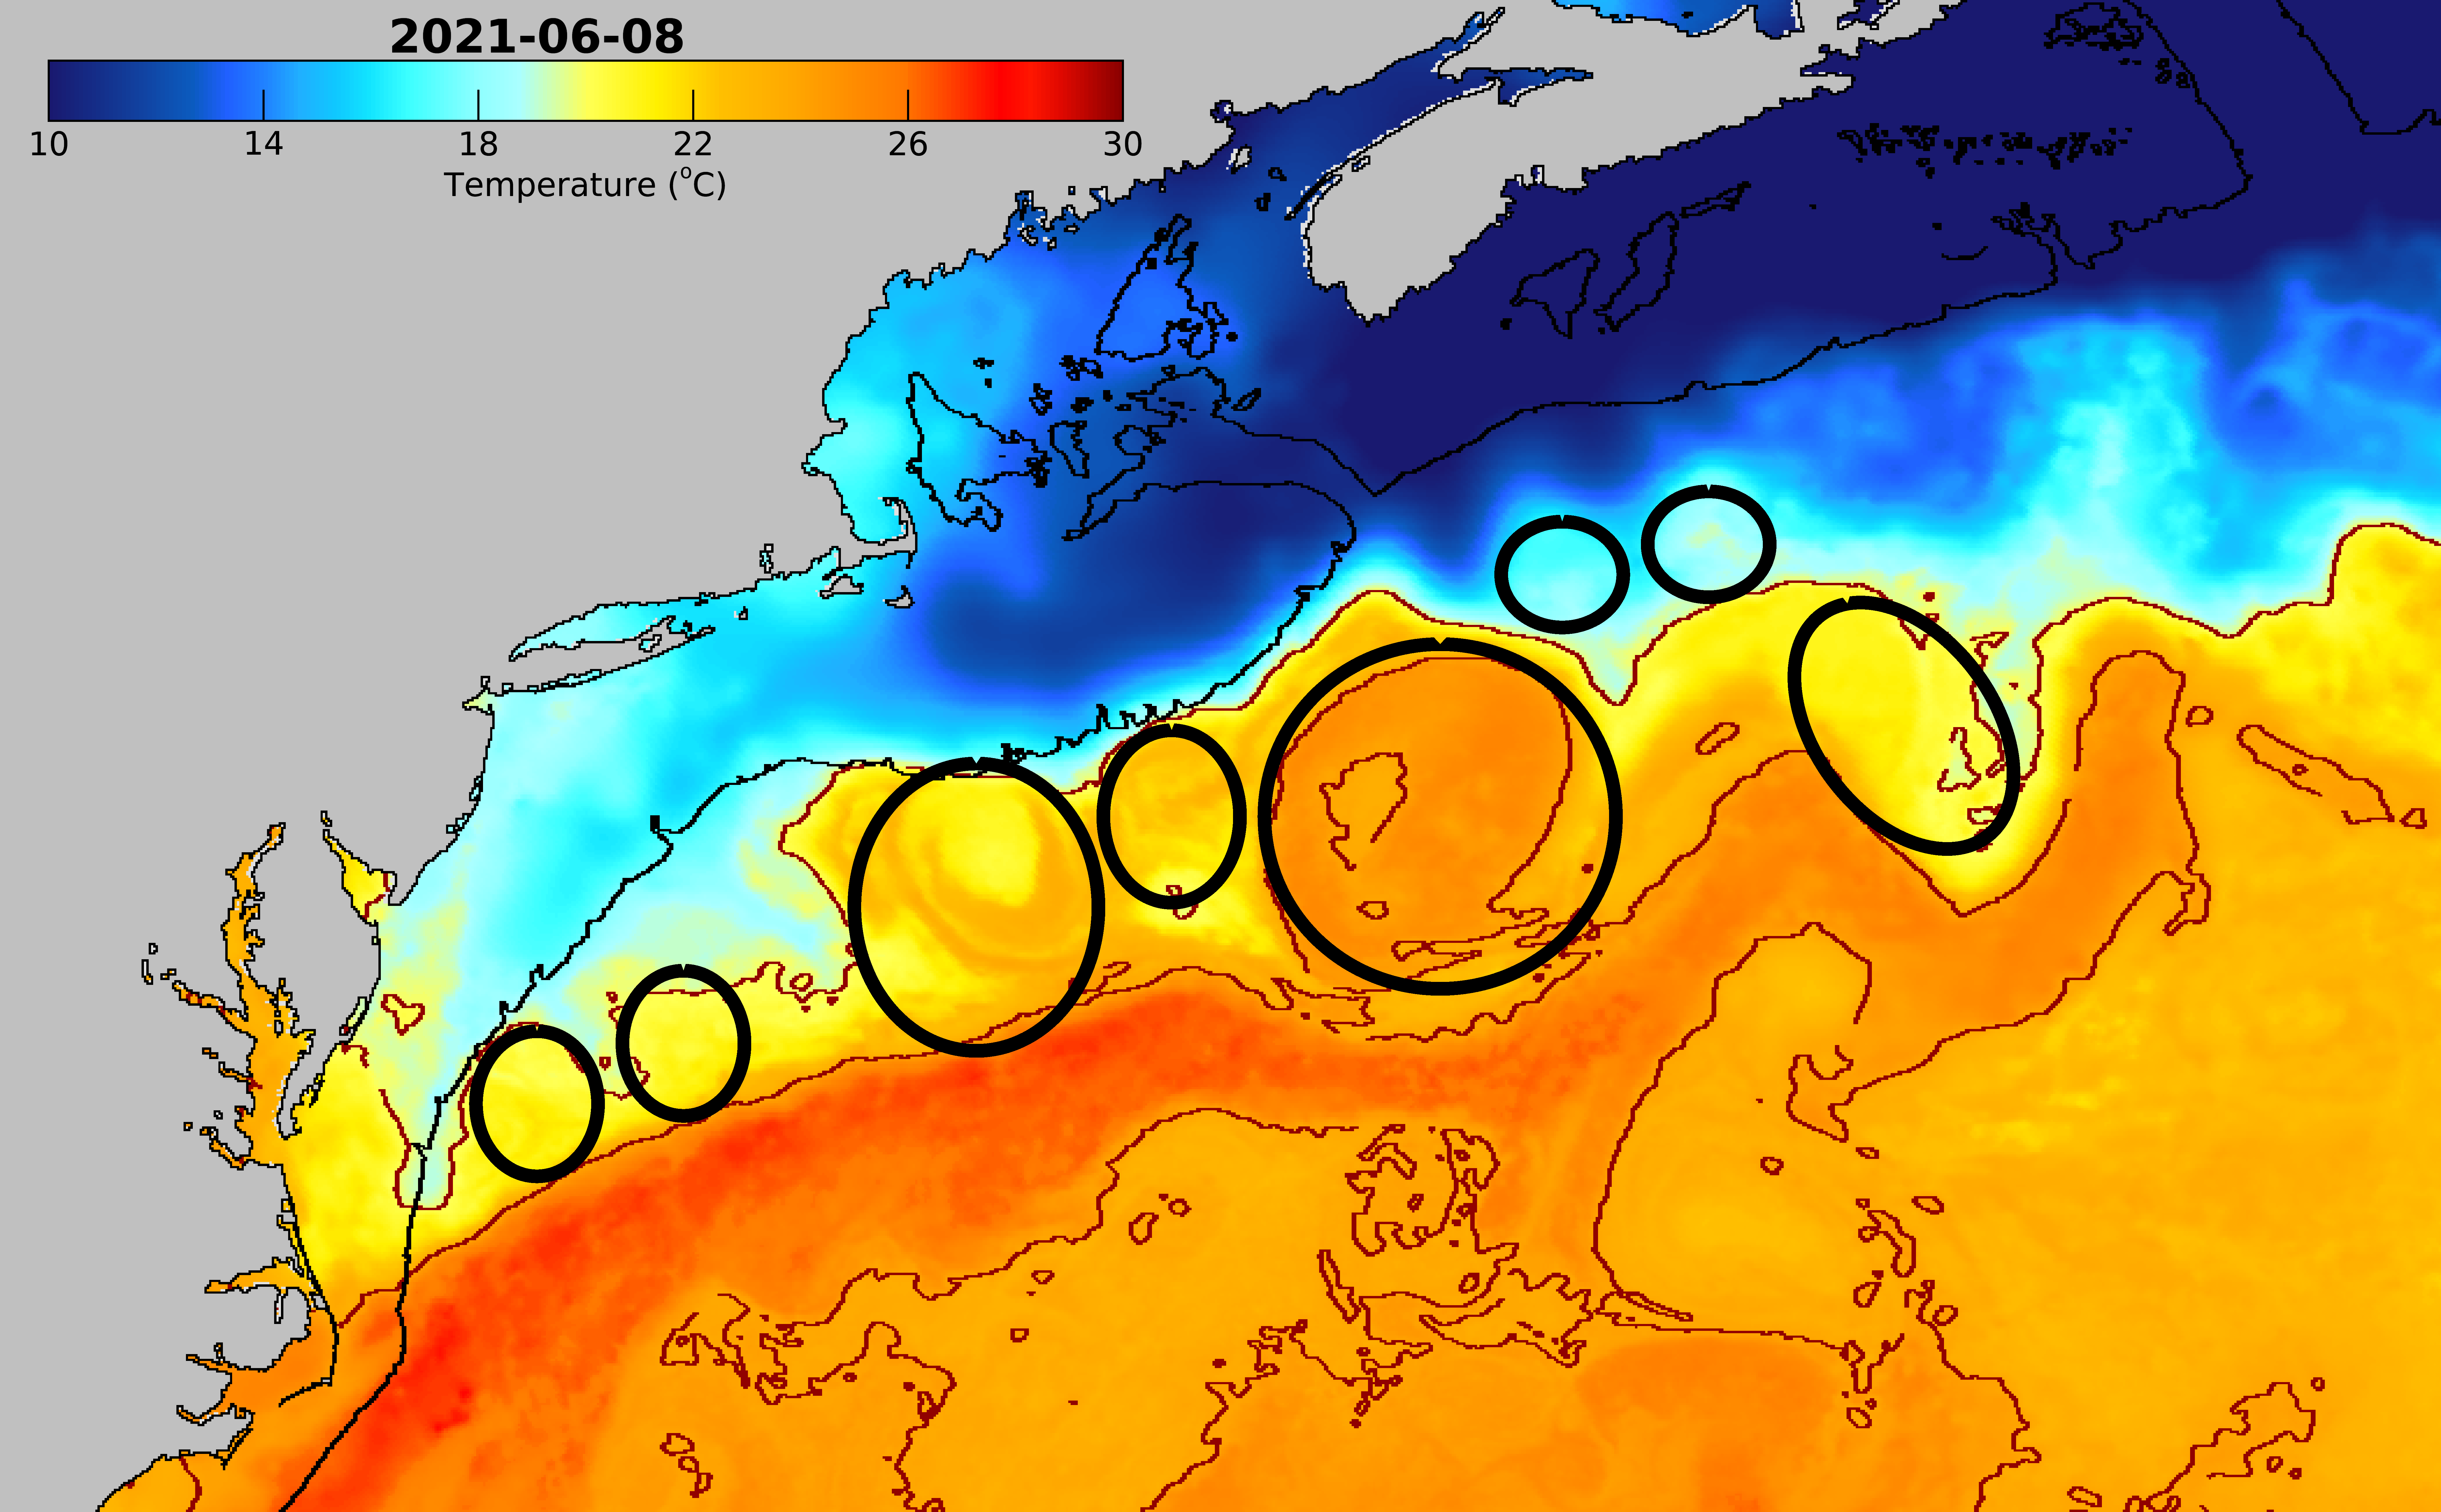
\includegraphics[width=0.49\linewidth]{images/D_20210608-MUR-SST-WCR} 

}

\caption{Warm core ring formation on the Northeast U.S. Shelf: Annual number of rings (left) and June 2021 rings (right), where the black line is the 200 m isobath (the shelf break) and the red lines are the 20 and 24 degree isotherms.}\label{fig:wcr}
\end{figure}

When warm core rings and eddies interact with the continental slope they
can transport warm, salty water to the continental shelf
{[}\protect\hyperlink{ref-chen_mesoscale_2022}{21}{]}, and this is now
happening more frequently
{[}\protect\hyperlink{ref-gawarkiewicz_changing_2018}{20},\protect\hyperlink{ref-gawarkiewicz_increasing_nodate}{22}{]}.
These interactions can be significant contributors to marine heatwaves
in the Mid-Atlantic Bight
{[}\protect\hyperlink{ref-chen_mesoscale_2022}{21},\protect\hyperlink{ref-gawarkiewicz_characteristics_2019}{23}{]}
as well as the movement of shelf-break species inshore
{[}\protect\hyperlink{ref-gawarkiewicz_changing_2018}{20},\protect\hyperlink{ref-potter_horizontal_2011}{24},\protect\hyperlink{ref-worm_predator_2003}{25}{]}.

Changes in ocean temperature and circulation alter habitat features such
as the seasonal cold pool, a 20--60 m thick band of cold, relatively
uniform near-bottom water that persists from spring to fall over the mid
and outer shelf of the MAB and southern flank of Georges Bank
{[}\protect\hyperlink{ref-lentz_seasonal_2017}{26},\protect\hyperlink{ref-chen_seasonal_2018}{27}{]}.
The cold pool plays an essential role in the structuring of the MAB
ecosystem. It is a reservoir of nutrients that feeds phytoplankton
productivity, is essential fish spawning and nursery habitat, and
affects fish distribution and behavior
{[}\protect\hyperlink{ref-lentz_seasonal_2017}{26},\protect\hyperlink{ref-miles_offshore_2021}{28}{]}.
The average temperature of the cold pool is getting warmer over time
{[}\protect\hyperlink{ref-miller_state-space_2016}{29},\protect\hyperlink{ref-du_pontavice_incorporating_nodate}{30}{]},
the area is getting smaller
{[}\protect\hyperlink{ref-friedland_middle_2022}{31}{]}, and the
duration is getting shorter (Fig. \ref{fig:cold-pool}).

\begin{figure}

{\centering \includegraphics{docs/images/cold-pool-1} 

}

\caption{Seasonal cold pool indices: mean temperature within the cold pool, cold pool persistence, and spatial extent.}\label{fig:cold-pool}
\end{figure}

\hypertarget{ocean-acidification}{%
\paragraph{Ocean Acidification}\label{ocean-acidification}}

Ocean acidification (OA) has caused measured declines in global ocean
pH. On the Northeast Shelf, summer bottom pH (2007-2021) varied
spatially and temporally, ranging from 7.69-8.07 (Fig. \ref{fig:mab-oa},
left panel). The lowest pH values were recorded in western Long Island
Sound, and nearshore to mid-shelf waters off the coast of New Jersey. In
summer 2021, water column pH from the glider-based profiles ranged from
7.67-8.22 (Fig. \ref{fig:mab-oa}, right panel). The lowest pH occurred
in bottom waters, reaching minimum values in shallow waters typically
inhabited by Atlantic surfclams (27-56 m) in the southern flank of the
Hudson Canyon (mean pH = 7.80).

This seasonal pH minimum in the Mid-Atlantic is associated with cold
pool subsurface and bottom water, which is cut off from mixing with
surface water by strong stratification. Fall mixing and slope water
intrusions act to increase the pH in outer shelf waters
{[}\protect\hyperlink{ref-wrightfairbanks_autonomous_2020}{32}{]}.

\begin{figure}

{\centering 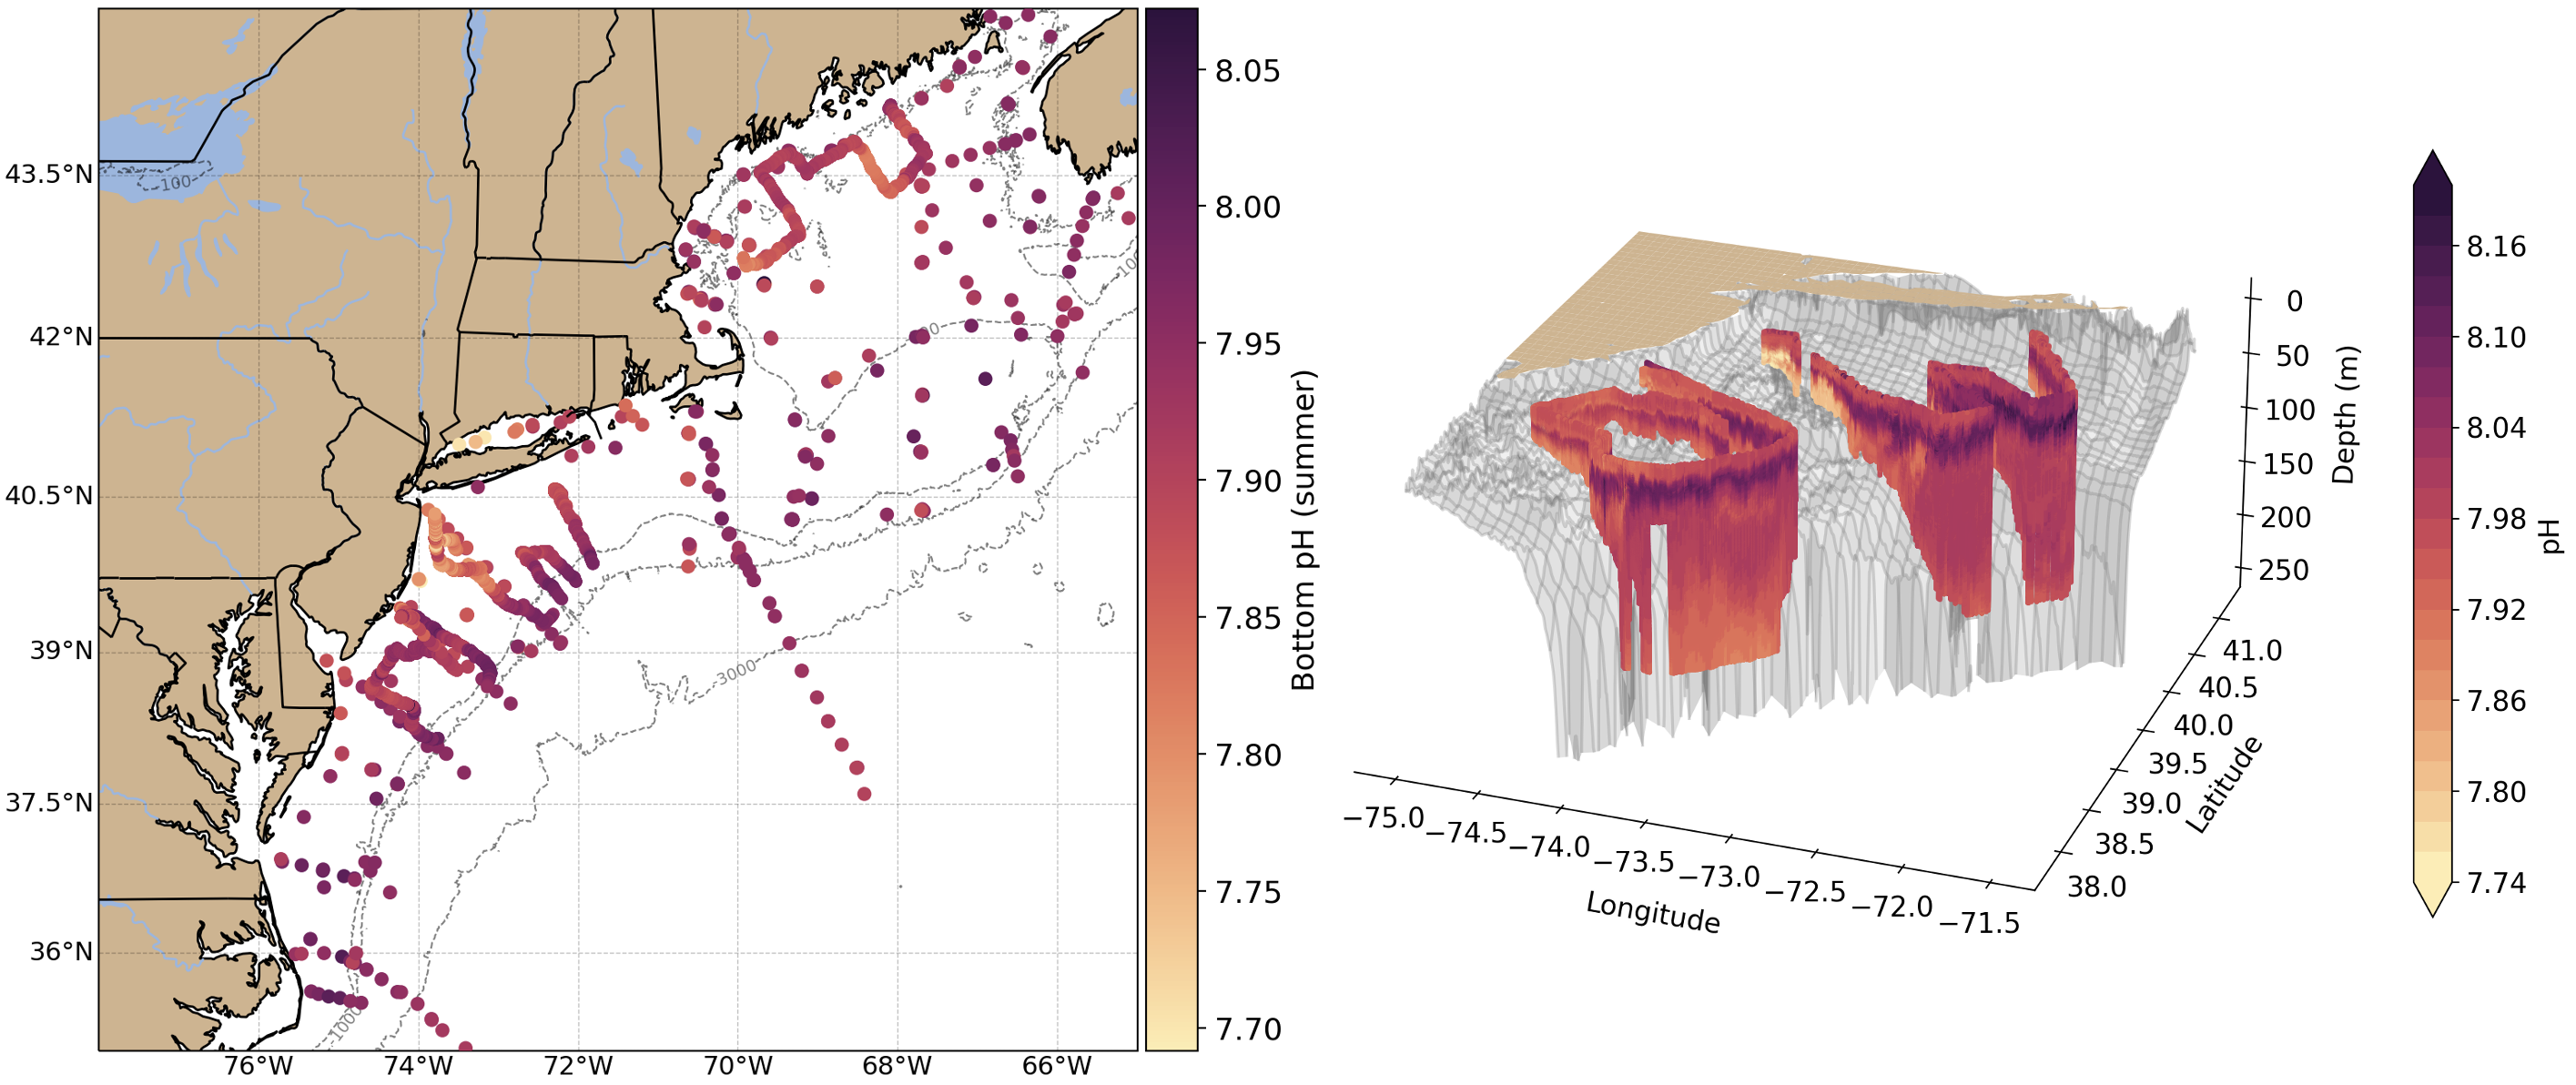
\includegraphics[width=0.8\linewidth]{images/Saba_Fig_SOE_MAFMC - Grace Saba} 

}

\caption{Left: Summer bottom pH collated from all quality-controlled vessel- and glider-based measurements from 2007-2021. Right: Glider-based pH profiles collected during summer 2021 in the Mid-Atlantic.}\label{fig:mab-oa}
\end{figure}

\hypertarget{ecosystem-productivity-indicators-phytoplankton-zooplankton-forage-fish-fish-condition}{%
\subsubsection{Ecosystem Productivity Indicators: phytoplankton,
zooplankton, forage fish, fish
condition}\label{ecosystem-productivity-indicators-phytoplankton-zooplankton-forage-fish-fish-condition}}

\hypertarget{phytoplankton}{%
\paragraph{Phytoplankton}\label{phytoplankton}}

Phytoplankton support the food web as the primary food source for
zooplankton and filter feeders such as shellfish. Numerous environmental
and oceanographic factors interact to drive the abundance, composition,
spatial distribution, and productivity of phytoplankton. In 2021, MAB
phytoplankton biomass (surface chlorophyll) was above average in winter,
but below average during the spring and summer months. Below average
phytoplankton biomass could be due to reduced nutrient flow to the
surface and/or increased grazing pressure. A short fall bloom was
detected in November. Primary productivity (the rate of photosynthesis)
was average to below average throughout 2021 (Fig.
\ref{fig:chl-weekly}).

\begin{figure}

{\centering \includegraphics{docs/images/chl-weekly-1} 

}

\caption{Weekly chlorophyll concentrations and primary productivity in the Mid-Atlantic are shown by the colored line for 2021 (dashed portion indicates preliminary data from a near real-time satellite source). The long-term mean is shown in black and shading indicates +/- 1 standard deviation.}\label{fig:chl-weekly}
\end{figure}

The seasonal cycle of phytoplankton size distribution shows that the
spring and fall bloom periods are dominated by larger-celled
microplankton, while smaller-celled nanoplankton dominate during the
warmer summer months. The proportion of the smallest phytoplankton,
picoplankton (0.2-2 microns), is relatively constant throughout the
year. In 2021, microplankton proportions were above average during the
winter and fall bloom periods, but below average for the summer months
(Fig. \ref{fig:weekly-phyto-size}).

\begin{figure}

{\centering \includegraphics{docs/images/weekly-phyto-size-1} 

}

\caption{The annual climatology (1998-2020) percent composition of the phytoplankton size classes in the Mid-Atlantic based on satellite observations in the shaded portions.  The 2021 proportions for the microplankton (>20 microns, green) and nanoplankton (2-20 microns, orange) are shown in the bold lines.}\label{fig:weekly-phyto-size}
\end{figure}

\hypertarget{zooplankton}{%
\paragraph{Zooplankton}\label{zooplankton}}

While zooplankton indicators could not be updated for this report due to
2020 survey disruptions and lags in sample processing, data up to 2019
showed long-term increasing trends of gelatinous zooplankton and krill
on the northeast shelf (see 2021 report\footnote{\url{https://repository.library.noaa.gov/view/noaa/29525}}).
Preliminary 2021 observations found the total volume of plankton caught
in the bongo net was significantly greater than the previous years due
to increased gelatinous zooplankton, predominantly salps (\emph{Thalia
democratica}). Unusually high concentrations of salps were found
throughout the Northeast shelf and in the Slope Sea during other summer
2021 scientific surveys, which may be associated with water mass
intrusions at the shelf break
{[}\protect\hyperlink{ref-madin_periodic_2006}{33},\protect\hyperlink{ref-deibel_predictability_2009}{34}{]}.
Salps are filter feeders feeding on phytoplankton and other small
particles and may have contributed to the below average phytoplankton
biomass in summer 2021 (Fig. \ref{fig:chl-weekly}).

\hypertarget{forage-fish-energy-content}{%
\paragraph{Forage Fish Energy
Content}\label{forage-fish-energy-content}}

Nutritional value (energy content) of juvenile and adult forage fish as
prey is related to environmental conditions, fish growth, and
reproductive cycles. Forage energy density measurements from NEFSC trawl
surveys 2017-2021 are building toward a time series to evaluate trends
(Fig. \ref{fig:energy-density}). Limited data from the spring 2020
survey, and complete spring 2021 survey measurements were consistent
with previous reports: the energy density of Atlantic herring was almost
half the value (5.69 +/- 0.07 kJ/g wet weight) reported in earlier
studies (10.6-9.4 kJ/ g wet weight). Silver hake, longfin squid
(\emph{Loligo} in figure) and shortfin squid (\emph{Illex} in figure)
were also lower than previous estimates
{[}\protect\hyperlink{ref-steimle_energy_1985}{35},\protect\hyperlink{ref-lawson_important_1998}{36}{]}.
Energy density of alewife, butterfish, sand lance, and Atlantic mackerel
varies seasonally, with seasonal estimates both higher and lower than
estimates from previous decades.

\begin{figure}

{\centering \includegraphics{docs/images/energy-density-1} 

}

\caption{Forage fish energy density mean and standard deviation by season and year, compared with 1980s (solid line; Steimle and Terranove 1985) and 1990s (dashed line; Lawson et al. 1998) values.}\label{fig:energy-density}
\end{figure}

\hypertarget{fish-condition}{%
\paragraph{Fish Condition}\label{fish-condition}}

The health and well being of individual fish can be related to body
shape condition indices (i.e., weight at a given length) such as
relative condition index, which is the ratio of observed weight to
predicted weight based on length
{[}\protect\hyperlink{ref-le_cren_length-weight_1951}{37}{]}. Heavier
and fatter fish at a given length have higher relative condition which
is expected to improve growth, reproductive output, and survival. A
pattern of generally good condition was observed across many MAB species
prior to 2000, followed by a period of generally poor condition from
2001-2010, with a mix of good and poor condition 2011-2019. However,
most species in the MAB had below average or poor condition again in
2021 (Fig. \ref{fig:mab-cf}). Preliminary results of synthetic analyses
show that changes in temperature, zooplankton, fishing pressure, and
population size influence the condition of different fish species.

\begin{figure}

{\centering 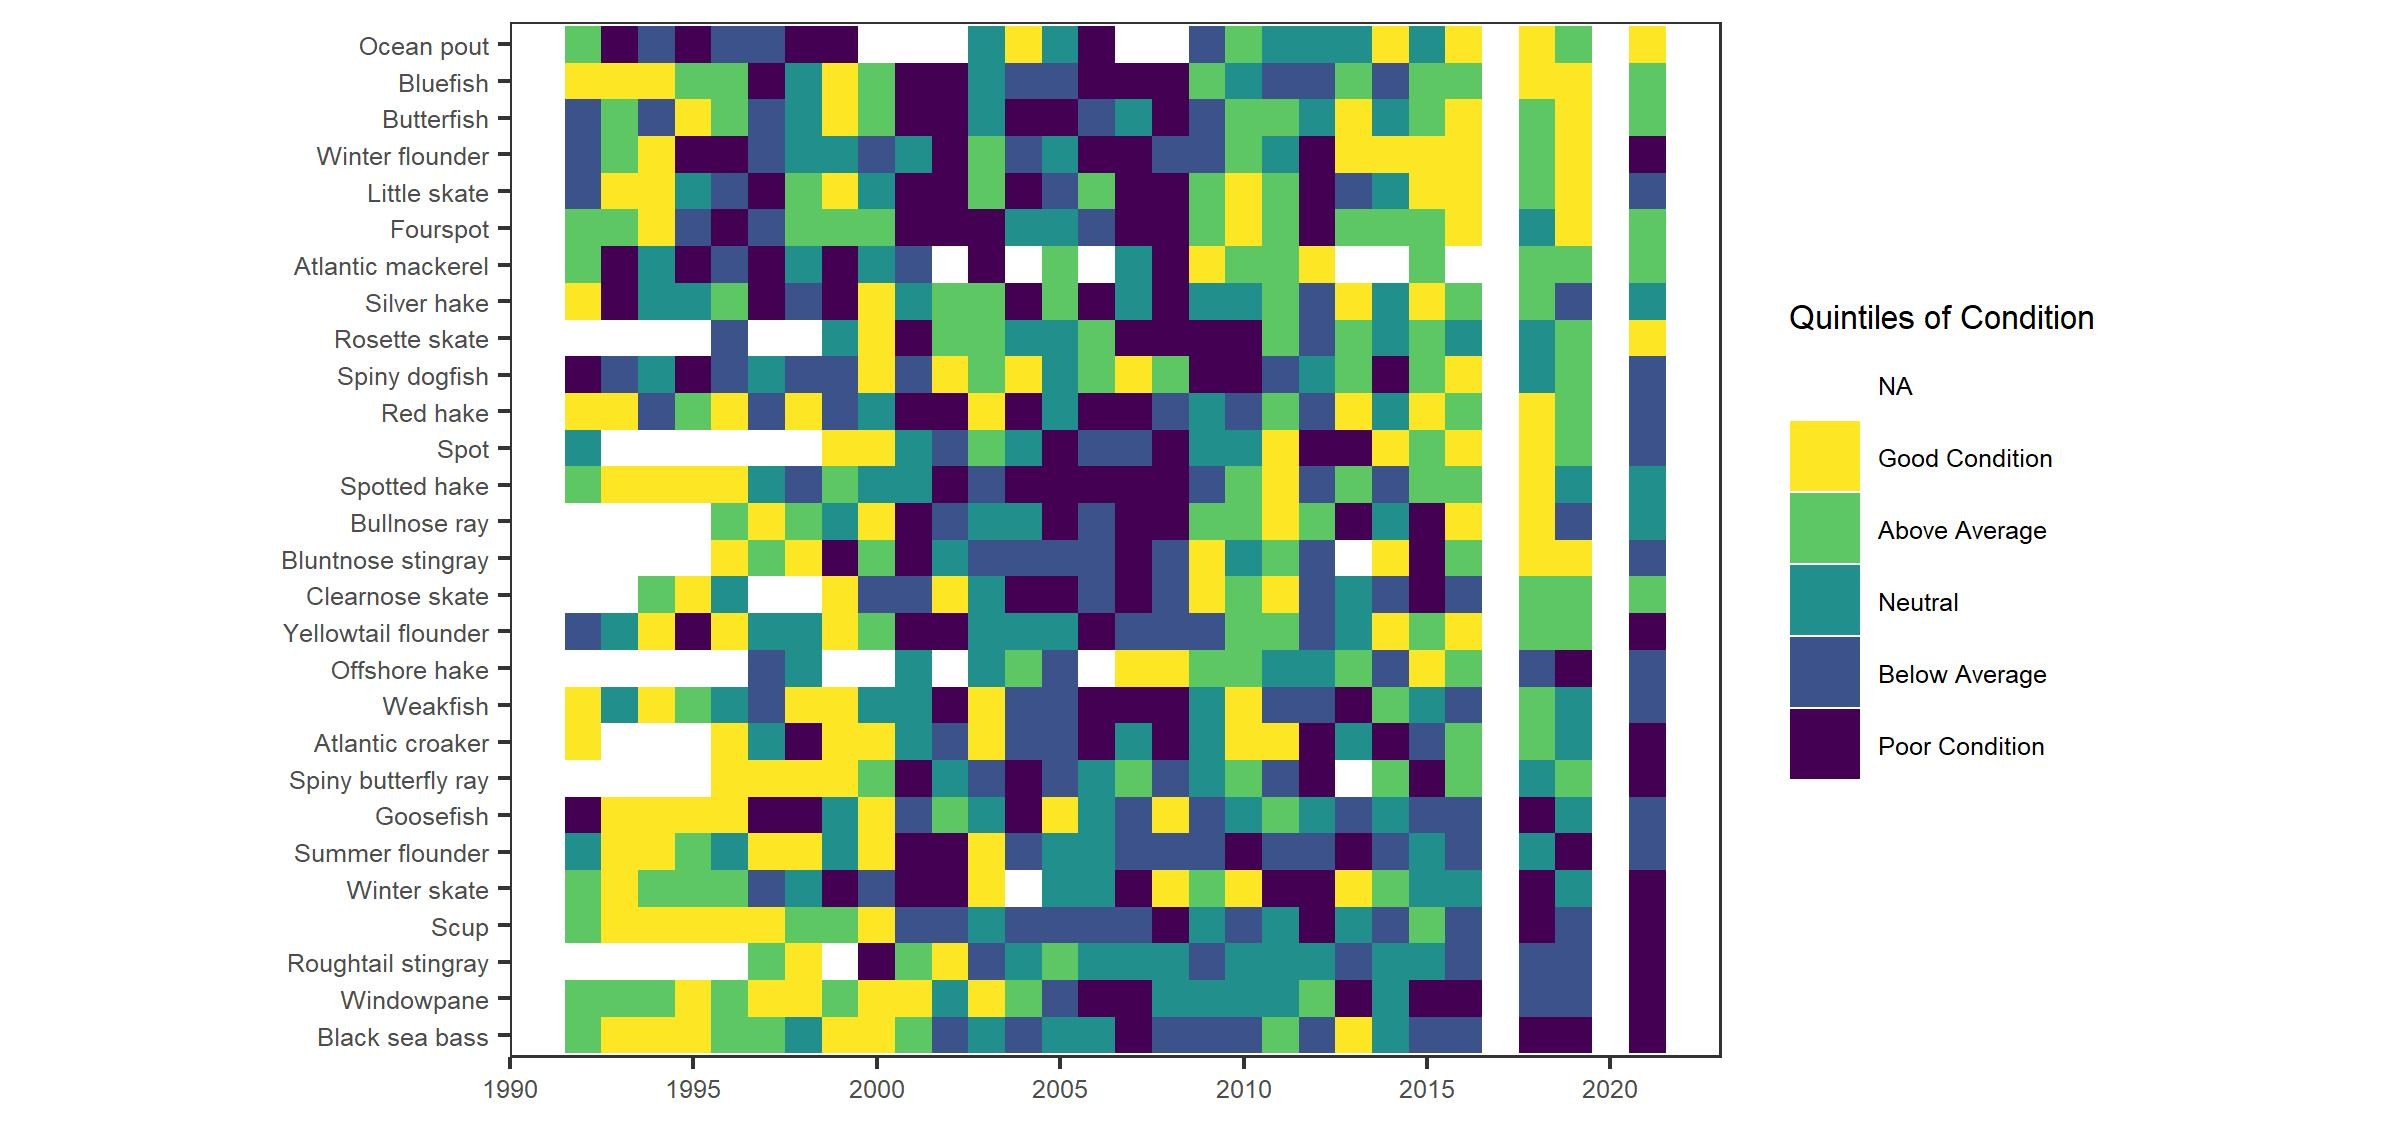
\includegraphics[width=1\linewidth]{images/MAB_Condition_allsex_2022_viridis} 

}

\caption{Condition factor for fish species in the MAB based on fall NEFSC bottom trawl survey data. MAB data are missing for 2017 due to survey delays, and no survey was conducted in 2020.}\label{fig:mab-cf}
\end{figure}

\hypertarget{fish-productivity}{%
\paragraph{Fish Productivity}\label{fish-productivity}}

We describe patterns of aggregate fish productivity in the Mid-Atlantic
with the small fish per large fish anomaly indicator, derived from NEFSC
bottom trawl survey data (Fig. \ref{fig:productivity-anomaly}). The
indicator shows that productivity has been declining in this region
since 2010.

\begin{figure}

{\centering \includegraphics{docs/images/productivity-anomaly-1} 

}

\caption{Small fish per large fish biomass anomaly in the Mid-Atlantic Bight. The summed anomaly across species is shown by the black line.}\label{fig:productivity-anomaly}
\end{figure}

\hypertarget{ecosystem-structure-indicators-distribution-shifts-diversity-predators}{%
\subsubsection{Ecosystem Structure Indicators: distribution shifts,
diversity,
predators}\label{ecosystem-structure-indicators-distribution-shifts-diversity-predators}}

As noted in the \protect\hyperlink{implications}{Landings Implications
section above}, stocks are shifting distribution throughout the region.
In aggregate, fish stocks are moving northeast along the shelf and into
deeper waters.

Zooplankton diversity was increasing in the MAB as of 2019, while adult
fish diversity indices appear stable over time, with current values
within one standard deviation from most historic estimates (see
\protect\hyperlink{ecological-diversity}{Diversity Indicators section,
above}).

New indicators for shark populations, combined with information on gray
seals (see \protect\hyperlink{protected-species}{Protected Species
Implications section, above}), suggests predator populations range from
stable (sharks, Fig. \ref{fig:hms-cpue-sharks}) to increasing (seals) in
the MAB. Stable predator populations suggest stable predation pressure
on managed species, but increasing predator populations may reflect
increasing predation pressure.

\begin{figure}

{\centering \includegraphics{docs/images/hms-cpue-sharks-1} 

}

\caption{Estimated number of sharks per unit effort from Highly Migratory Species Pelagic Observer Program data.}\label{fig:hms-cpue-sharks}
\end{figure}

Stock status is mixed for Atlantic Highly Migratory Species (HMS) stocks
(including sharks, swordfish, billfish, and tunas) occurring in the
Mid-Atlantic region. While there are several HMS species considered to
be overfished or that have unknown stock status, the population status
for some managed Atlantic sharks and tunas is at or above the biomass
target (Fig. \ref{fig:hms-stock-status} ), suggesting the potential for
robust predator populations among these managed species.

\begin{figure}

{\centering \includegraphics{docs/images/hms-stock-status-1} 

}

\caption{Summary of single species status for HMS stocks; key to species names at https://noaa-edab.github.io/tech-doc/atlantic-highly-migratory-species-stock-status.html.}\label{fig:hms-stock-status}
\end{figure}

As noted in the \protect\hyperlink{protected-species}{Protected Species
section}, gray seal populations are increasing. Harbor and gray seals
occupying New England waters are generalist predators that consume more
than 30 different prey species. An evaluation of hard parts found in
seal stomachs showed that harbor and gray seals predominantly exploit
abundant demersal fish species (i.e., red, white, and silver hake).
Other relatively abundant prey species found in hard-part remains
include sand lance, yellowtail flounder, four-spotted flounder, Gulf
Stream flounder, haddock, herring, redfish, and squids.

A recent stable isotope study utilizing gray seal scat samples obtained
from Massachusetts habitats showed individual gray seals can specialize
on particular prey. It also found that gray seals vary their diet
seasonally, focusing on demersal inshore species prior to the spring
molt, and offshore species such as sand lance after molting. DNA studies
on gray seal diet in Gulf of Maine and Massachusetts waters found spiny
dogfish and Jonah crab present in gray seal scat samples. Skate and crab
remains were also found in gray seal stomach remains. In contrast to
direct feeding, it is uncertain if the presence of skates and crabs is
due to secondary consumption or scavenging.

\hypertarget{habitat-risk-indicators-habitat-assessments-submerged-aquatic-vegetation-estuarine-habitat-quality-fishing-gear-impacts}{%
\subsubsection{Habitat Risk Indicators: habitat assessments, submerged
aquatic vegetation, estuarine habitat quality, fishing gear
impacts}\label{habitat-risk-indicators-habitat-assessments-submerged-aquatic-vegetation-estuarine-habitat-quality-fishing-gear-impacts}}

\hypertarget{habitat-assessments}{%
\paragraph{Habitat Assessments}\label{habitat-assessments}}

The Northeast Regional Marine Fish Habitat Assessment (NRHA) is a
collaborative effort to describe and characterize estuarine, coastal,
and offshore fish habitat distribution, abundance, and quality in the
Northeast. This includes mapping inshore and offshore habitat types used
by focal fish species, summarizing impacts of habitat climate
vulnerability on these species, modeling predicted future species
distributions, and developing a publicly accessible decision support
tool to visualize these results. This is a three-year project led by the
New England and Mid-Atlantic Fishery Management Councils in
collaboration with many partners including NOAA Fisheries, and will be
completed in July 2022\footnote{\url{https://www.mafmc.org/nrha}}.

As part of the NRHA work, climate vulnerability information from NOAA's
Habitat Climate Vulnerability Assessment
{[}\protect\hyperlink{ref-farr_assessment_2021}{38}{]} and the Northeast
Fish and Shellfish Climate Vulnerability Assessment
{[}\protect\hyperlink{ref-hare_vulnerability_2016}{39}{]}\footnote{\url{https://www.fisheries.noaa.gov/new-england-mid-atlantic/climate/northeast-vulnerability-assessment}}
is synthesized for approximately 70 species in the northeast region. For
example, black sea bass, scup, and summer founder have been linked to
several highly vulnerable nearshore habitats from salt marsh, submerged
aquatic vegetation, and shallow estuarine and marine reefs. Details on
highly vulnerable habitats with linkages to a variety of species,
including which life stages have different levels of dependence on a
particular habitat, are available in a detailed table\footnote{\url{https://noaa-edab.github.io/ecodata/Hab_table}}.

\hypertarget{submerged-aquatic-vegetation}{%
\paragraph{Submerged Aquatic
Vegetation}\label{submerged-aquatic-vegetation}}

Submerged aquatic vegetation (SAV) is designated as a Habitat Area of
Particular Concern (HAPC) for summer flounder and is important habitat
for many fish species, particularly during vulnerable juvenile stages.
Increased SAV coverage (including wild celery, water stargrass, and
hydrilla) in the tidal fresh areas of the Chesapeake Bay (Fig.
\ref{fig:sav}) has been attributed to restoration efforts. This
ecosystem engineering has improved water quality, promoting further
expansions of SAV meadows. However, in the higher salinity region near
the mouth of the Chesapeake Bay (Fig. \ref{fig:sav}), increased water
temperatures, especially during the summer, have led to a decline in
eelgrass coverage.

\begin{figure}

{\centering \includegraphics{docs/images/sav-1} 

}

\caption{Submerged Aquatic Vegetation (SAV) coverage in tidal fresh and high salinity regions of the Chesapeake Bay.}\label{fig:sav}
\end{figure}

\hypertarget{estuarine-habitat-quality-chesapeake-bay}{%
\paragraph{Estuarine Habitat Quality (Chesapeake
Bay)}\label{estuarine-habitat-quality-chesapeake-bay}}

Many important MAFMC managed species (e.g., summer flounder, scup, black
sea bass, and bluefish) use estuarine habitats as nurseries or are
considered estuarine and nearshore coastal-dependent, and interact with
other important estuarine-dependent species (e.g., striped bass and
menhaden). An integrated measure of multiple water quality criteria
shows a significantly increasing proportion of Chesapeake Bay waters
meeting or exceeding EPA water quality standards over time
({[}\protect\hyperlink{ref-zhang_chesapeake_2018}{40}{]}; Fig.
\ref{fig:cb-attainment}). This pattern was statistically linked to total
nitrogen reduction, indicating responsiveness of water quality status to
management actions implemented to reduce nutrients. Water quality trends
and status may be used to inform aquaculture siting decisions in
Chesapeake Bay.

\begin{figure}

{\centering \includegraphics{docs/images/cb-attainment-1} 

}

\caption{Water quality attainment in Chesapeake Bay following rolling three year assessment periods.}\label{fig:cb-attainment}
\end{figure}

\hypertarget{fishing-gear-impacts}{%
\paragraph{Fishing Gear Impacts}\label{fishing-gear-impacts}}

Estimates of the impacts of fishing gear on habitat are available
through the habitat section of the Northeast Ocean Data
Portal\footnote{\url{https://www.northeastoceandata.org/data-explorer/}}.
The data portal hosts selected outputs from the Northeast Fishing
Effects Model which combines seafloor data (sediment type, energy
regime) with fishing effort data to generate percent habitat disturbance
estimates in space and time. More detailed information can be found in
the Synthetic Indicator Catalog.\footnote{\url{https://noaa-edab.github.io/catalog/northeast-fishing-effects-model.html}}

\hypertarget{implications-6}{%
\subsubsection{Implications}\label{implications-6}}

\hypertarget{links-between-climate-change-and-managed-species}{%
\paragraph{Links between climate change and managed
species}\label{links-between-climate-change-and-managed-species}}

Estuarine, nearshore, and offshore habitats support many life stages of
state and federally managed species, and are highly vulnerable to
climate change. Below we highlight how recently observed habitat changes
affect several key managed species in Chesapeake Bay and in both
nearshore and offshore waters of the MAB. Overall, multiple drivers
interact differently for each species, producing a range of population
impacts.

\hypertarget{striped-bass}{%
\subparagraph{\texorpdfstring{\emph{Striped
Bass}}{Striped Bass}}\label{striped-bass}}

Increasing water temperatures in Chesapeake Bay have negative impacts on
striped bass at all life stages, although impovements in water quality
mitigate some impacts. Declining recruitment since 2000 is associated
with higher winter and spring water temperatures and lower freshwater
flows, which compress the reproductive season, cause production of
zooplankton prey earlier in the season before striped bass larvae are
feeding, and reduce concentration of zooplankton prey in larval habitat.

In 2021, average summer water temperatures combined with better
dissolved oxygen conditions likely improved habitat quality for larger
juvenile and adult striped bass in the summer. The expansion of
submerged aquatic vegetation meadows in the tidal fresh region of the
Chesapeake Bay (Fig. \ref{fig:sav}) is likely benefiting species like
striped bass who use this as spawning and nursery habitat in the spring.
However, similar to 2020, the warm winter in 2021 may have reduced
larval survival, despite the average spring temperatures and high spring
flows, which represent favorable conditions for striped bass recruitment
success.

Understanding habitat conditions can enhance recreational fishery
management. Maryland Department of Natural Resources is incorporating
habitat conditions into striped bass catch-and-release management,
including 1) a two-week summer closure directed at reducing
catch-and-release mortality\footnote{\url{https://dnr.maryland.gov/fisheries/Documents/StripedBass_regulations2022.pdf}}
as a substitute for harvest season reductions, and 2) the Striped Bass
Fishing Advisory\footnote{\url{https://dnr.maryland.gov/fisheries/Pages/SB_forecast.aspx}},
which lets anglers know the relative level of risk of released fish
dying due to high temperatures.

\hypertarget{blue-crabs}{%
\subparagraph{\texorpdfstring{\emph{Blue
Crabs}}{Blue Crabs}}\label{blue-crabs}}

Warmer winter temperatures may benefit Chesapeake Bay blue crabs, an
important commercial and forage species. Above-average fall and winter
temperatures in 2021 may have reduced overwintering mortality
{[}\protect\hyperlink{ref-bauer_temperature-_2010}{41}--\protect\hyperlink{ref-rome_linking_2005}{43}{]}
and contributed to increased productivity of blue crabs going into 2022.
Longer growth seasons are associated with increased production of blue
crabs and oysters in Chesapeake Bay. Blue crabs are moving northward
with warming temperatures and have been documented in the Gulf of Maine
{[}\protect\hyperlink{ref-johnson_savory_2015}{44}{]}, with implications
for both their management and for the inshore ecosystems.

\hypertarget{eastern-oyster}{%
\subparagraph{\texorpdfstring{\emph{Eastern
Oyster}}{Eastern Oyster}}\label{eastern-oyster}}

Oyster reefs provide habitat for several managed fish species including
juvenile black sea bass and summer flounder. Increased Chesapeake Bay
salinity has been linked to high juvenile oyster abundance
{[}\protect\hyperlink{ref-kimmel_relationship_2014}{45}{]}. In 2021,
high oyster spat set was predicted based on high summer
salinity\footnote{\url{https://content.buoybay.noaa.gov/sites/default/files/NCBOSeasonalSummary2021Summer.pdf}},
and was observed in Maryland during fall 2021. Virginia oyster
recruitment was at record levels 2019-2020 and was above average in
2021.

\hypertarget{summer-flounder-and-black-sea-bass}{%
\subparagraph{\texorpdfstring{\emph{Summer Flounder and Black Sea
Bass}}{Summer Flounder and Black Sea Bass}}\label{summer-flounder-and-black-sea-bass}}

The reduced amount of Chesapeake Bay water volume with low oxygen
(hypoxic volume) in June and July 2021 suggests better environmental
conditions during a critical period of juvenile production for key
species such as black sea bass and summer flounder. The increase in
hypoxic volume in the fall, however, may have been particularly harmful
as it coincided with above-average water temperatures. Additionally,
eelgrass in the higher salinity areas near the mouth of the Chesapeake
Bay (Fig. \ref{fig:sav}) is critical nursery habitat for summer
flounder, and recent declines seen in SAV coverage could negatively
impact recruitment survival.

\hypertarget{surfclam}{%
\subparagraph{\texorpdfstring{\emph{Surfclam}}{Surfclam}}\label{surfclam}}

Ocean acidification also has different implications, depending on the
species and life stage. Recent lab studies have found that surf clams
exhibited metabolic depression in a pH range of 7.46-7.28
{[}\protect\hyperlink{ref-pousse_energetic_2020}{46}{]}. Computer models
are in development to help determine the long term implications of
growth on surf clam populations. Aggregated data from 2007-2021 show
that summer bottom ocean pH (7.69-8.07, Fig. \ref{fig:mab-oa}) has not
yet reached the metabolic depression threshold observed for surfclams in
lab studies so far.

\hypertarget{northern-shortfin-squid}{%
\subparagraph{\texorpdfstring{\emph{Northern Shortfin
Squid}}{Northern Shortfin Squid}}\label{northern-shortfin-squid}}

Since 2017, extraordinarily high availability of northern shortfin squid
have been observed in the Mid-Atlantic, resulting in high fishery catch
per unit effort (CPUE) and early fishery closures. High instances of
squid catch near the shelf break are significantly related to low bottom
temperatures (\textless{} 10 degrees C), high salinity (
\textgreater35.6 psu), increased chlorophyll frontal activity as well as
the presence and orientation of warm core rings. Warm core rings are an
important contributor to squid availability, likely influencing habitat
conditions across different life stages. In particular, fishing effort
was concentrated on the eastern edge of warm core rings, which are
associated with upwelling and enhanced productivity.

\hypertarget{heatwave-impacts}{%
\paragraph{Heatwave impacts}\label{heatwave-impacts}}

While marine heatwaves lasting over days may disturb the marine
environment, long lasting events such as the warming in 2012 (Fig.
\ref{fig:heatwave}) can have significant impacts to the ecosystem
{[}\protect\hyperlink{ref-gawarkiewicz_characteristics_2019}{23}{]}. The
2012 heatwave affected the lobster fishery most notably, but other
species also shifted their geographic distributions and seasonal cycles
{[}\protect\hyperlink{ref-mills_fisheries_2013}{47}{]}. The 2012
heatwave was caused by a shift in the atmospheric Jet Stream, whereas
the 2017 marine heatwave in the Mid-Atlantic was associated with a
strong positive salinity anomaly and is likely related to cross-shelf
flow driven by the presence of a warm core ring adjacent to the
shelfbreak south of New England
{[}\protect\hyperlink{ref-gawarkiewicz_characteristics_2019}{23}{]}.
During the 2017 event, warm water fish typically found in the Gulf
Stream were caught in shallow waters near Block Island, RI
{[}\protect\hyperlink{ref-gawarkiewicz_changing_2018}{20}{]}. Ocean
temperatures in 2021 rivaled or exceeded the record temperatures in 2012
in some seasons, but the impacts to fisheries have yet to be determined.

\begin{figure}

{\centering \includegraphics{docs/images/heatwave-1} 

}

\caption{Marine heatwave cumulative intesity (left) and maximum intensity (right) in the Mid-Atlantic Bight.}\label{fig:heatwave}
\end{figure}

\hypertarget{cold-pool-impacts}{%
\paragraph{Cold pool impacts}\label{cold-pool-impacts}}

Changes in the cold pool habitat can affect species distribution,
recruitment, and migration timing for multiple federally managed
species. Southern New England-Mid Atlantic yellowtail flounder
recruitment and settlement are related to the strength of the cold pool
{[}\protect\hyperlink{ref-miller_state-space_2016}{29}{]}. The
settlement of pre-recruits during the cold pool event represents a
bottleneck in yellowtail life history, during which a local and
temporary increase in bottom temperature negatively impacts the survival
of the settlers. Including the effect of cold pool variations on
yellowtail recruitment reduced retrospective patterns and improved the
skill of short-term forecasts in a stock assessment model
{[}\protect\hyperlink{ref-miller_state-space_2016}{29},\protect\hyperlink{ref-du_pontavice_incorporating_nodate}{30}{]}.
The cold pool also provides habitat for the ocean quahog
{[}\protect\hyperlink{ref-friedland_middle_2022}{31},\protect\hyperlink{ref-powell_ocean_2020}{48}{]}.
Growth rates of ocean quahogs in the MAB (southern portion of their
range) have increased over the last 200 years whereas little to no
change has been documented in the northern portion of their range in
southern New England, likely a response to a warming and shrinking cold
pool {[}\protect\hyperlink{ref-pace_two-hundred_2018}{49}{]}.

\hypertarget{distribution-shift-impacts}{%
\paragraph{Distribution shift
impacts}\label{distribution-shift-impacts}}

Trends for a suite of 48 commercially or ecologically important fish
species along the entire Northeast Shelf continue to show movement
towards the northeast and generally into deeper water (Fig.
\ref{fig:species-dist}). We hope to expand this analysis beyond fish.
Marine mammal distribution maps are available online\footnote{\url{https://www.nefsc.noaa.gov/AMAPPSviewer/}};
updated maps and trends are currently being developed.

Shifting species distributions alter both species interactions and
fishery interactions. In particular, shifting species distributions can
alter expected management outcomes from spatial allocations and bycatch
measures based on historical fish and protected species distributions.

\hypertarget{ecosystem-productivity-change-impacts}{%
\paragraph{Ecosystem productivity change
impacts}\label{ecosystem-productivity-change-impacts}}

Climate and associated changes in the physical environment affect
ecosystem productivity, with warming waters increasing the rate of
photosynthesis at the base of the food web. However, increased summer
production in the MAB may not translate to increased fish biomass
because smaller phytoplankton dominate in this season.

While krill and large gelatinous zooplankton are increasing over time,
smaller zooplankton are periodically shifting abundance between the
larger, more nutritious \emph{Calanus finmarchicus} and smaller bodied
copepods with no apparent overall trend. The nutritional content of
larger bodied forage fish and squid changes seasonally in response to
ecosystem conditions, with apparent declines in energy density for
Atlantic herring and \emph{Illex} squid relative to the 1980s, but
similar energy density for other forage species. Some of these factors
are now being linked to the relative condition of managed fish.

The apparent decline in productivity across multiple managed species in
the MAB, along with low fish condition for many species in 2021, also
suggest changing ecosystem productivity at multiple levels. During the
1990s and early 2000s high relative abundance of smaller bodied copepods
and a lower relative abundance of \emph{Calanus finmarchicus} was
associated with regime shifts to lower fish recruitment
{[}\protect\hyperlink{ref-perretti_regime_2017}{50}{]}. The
unprecedented climate signals along with the trends toward lower
productivity across multiple managed species indicate a need to
continually evaluate whether management reference points remain
appropriate, and to evaluate if ecosystem regime shifts have occurred or
reorganization is in progress.

\hypertarget{other-ocean-uses-offshore-wind}{%
\subsection{Other Ocean Uses: Offshore
Wind}\label{other-ocean-uses-offshore-wind}}

\hypertarget{indicators-development-timeline-revenue-in-lease-areas-coastal-community-vulnerability}{%
\subsubsection{Indicators: development timeline, revenue in lease areas,
coastal community
vulnerability}\label{indicators-development-timeline-revenue-in-lease-areas-coastal-community-vulnerability}}

As of February 2022, 24 offshore wind development projects are proposed
for construction over the next decade in the Northeast (timelines and
project data are based on Tables E-2, E-4, and E-4-2 of South Fork Wind
Farm Final Environmental Impact Statement). Offshore wind areas are
anticipated to cover more than 1.7 million acres by 2030 in the Greater
Atlantic region (Fig. \ref{fig:wind-proposed-dev}). Beyond 2030 values
include acreage for the NY Wind Energy Areas (WEA) and Gulf of Maine
Area of Interest for floating research array.

\begin{figure}

{\centering \includegraphics{docs/images/wind-proposed-dev-1} 

}

\caption{Proposed wind development on the northeast shelf.}\label{fig:wind-proposed-dev}
\end{figure}

\begin{figure}

{\centering 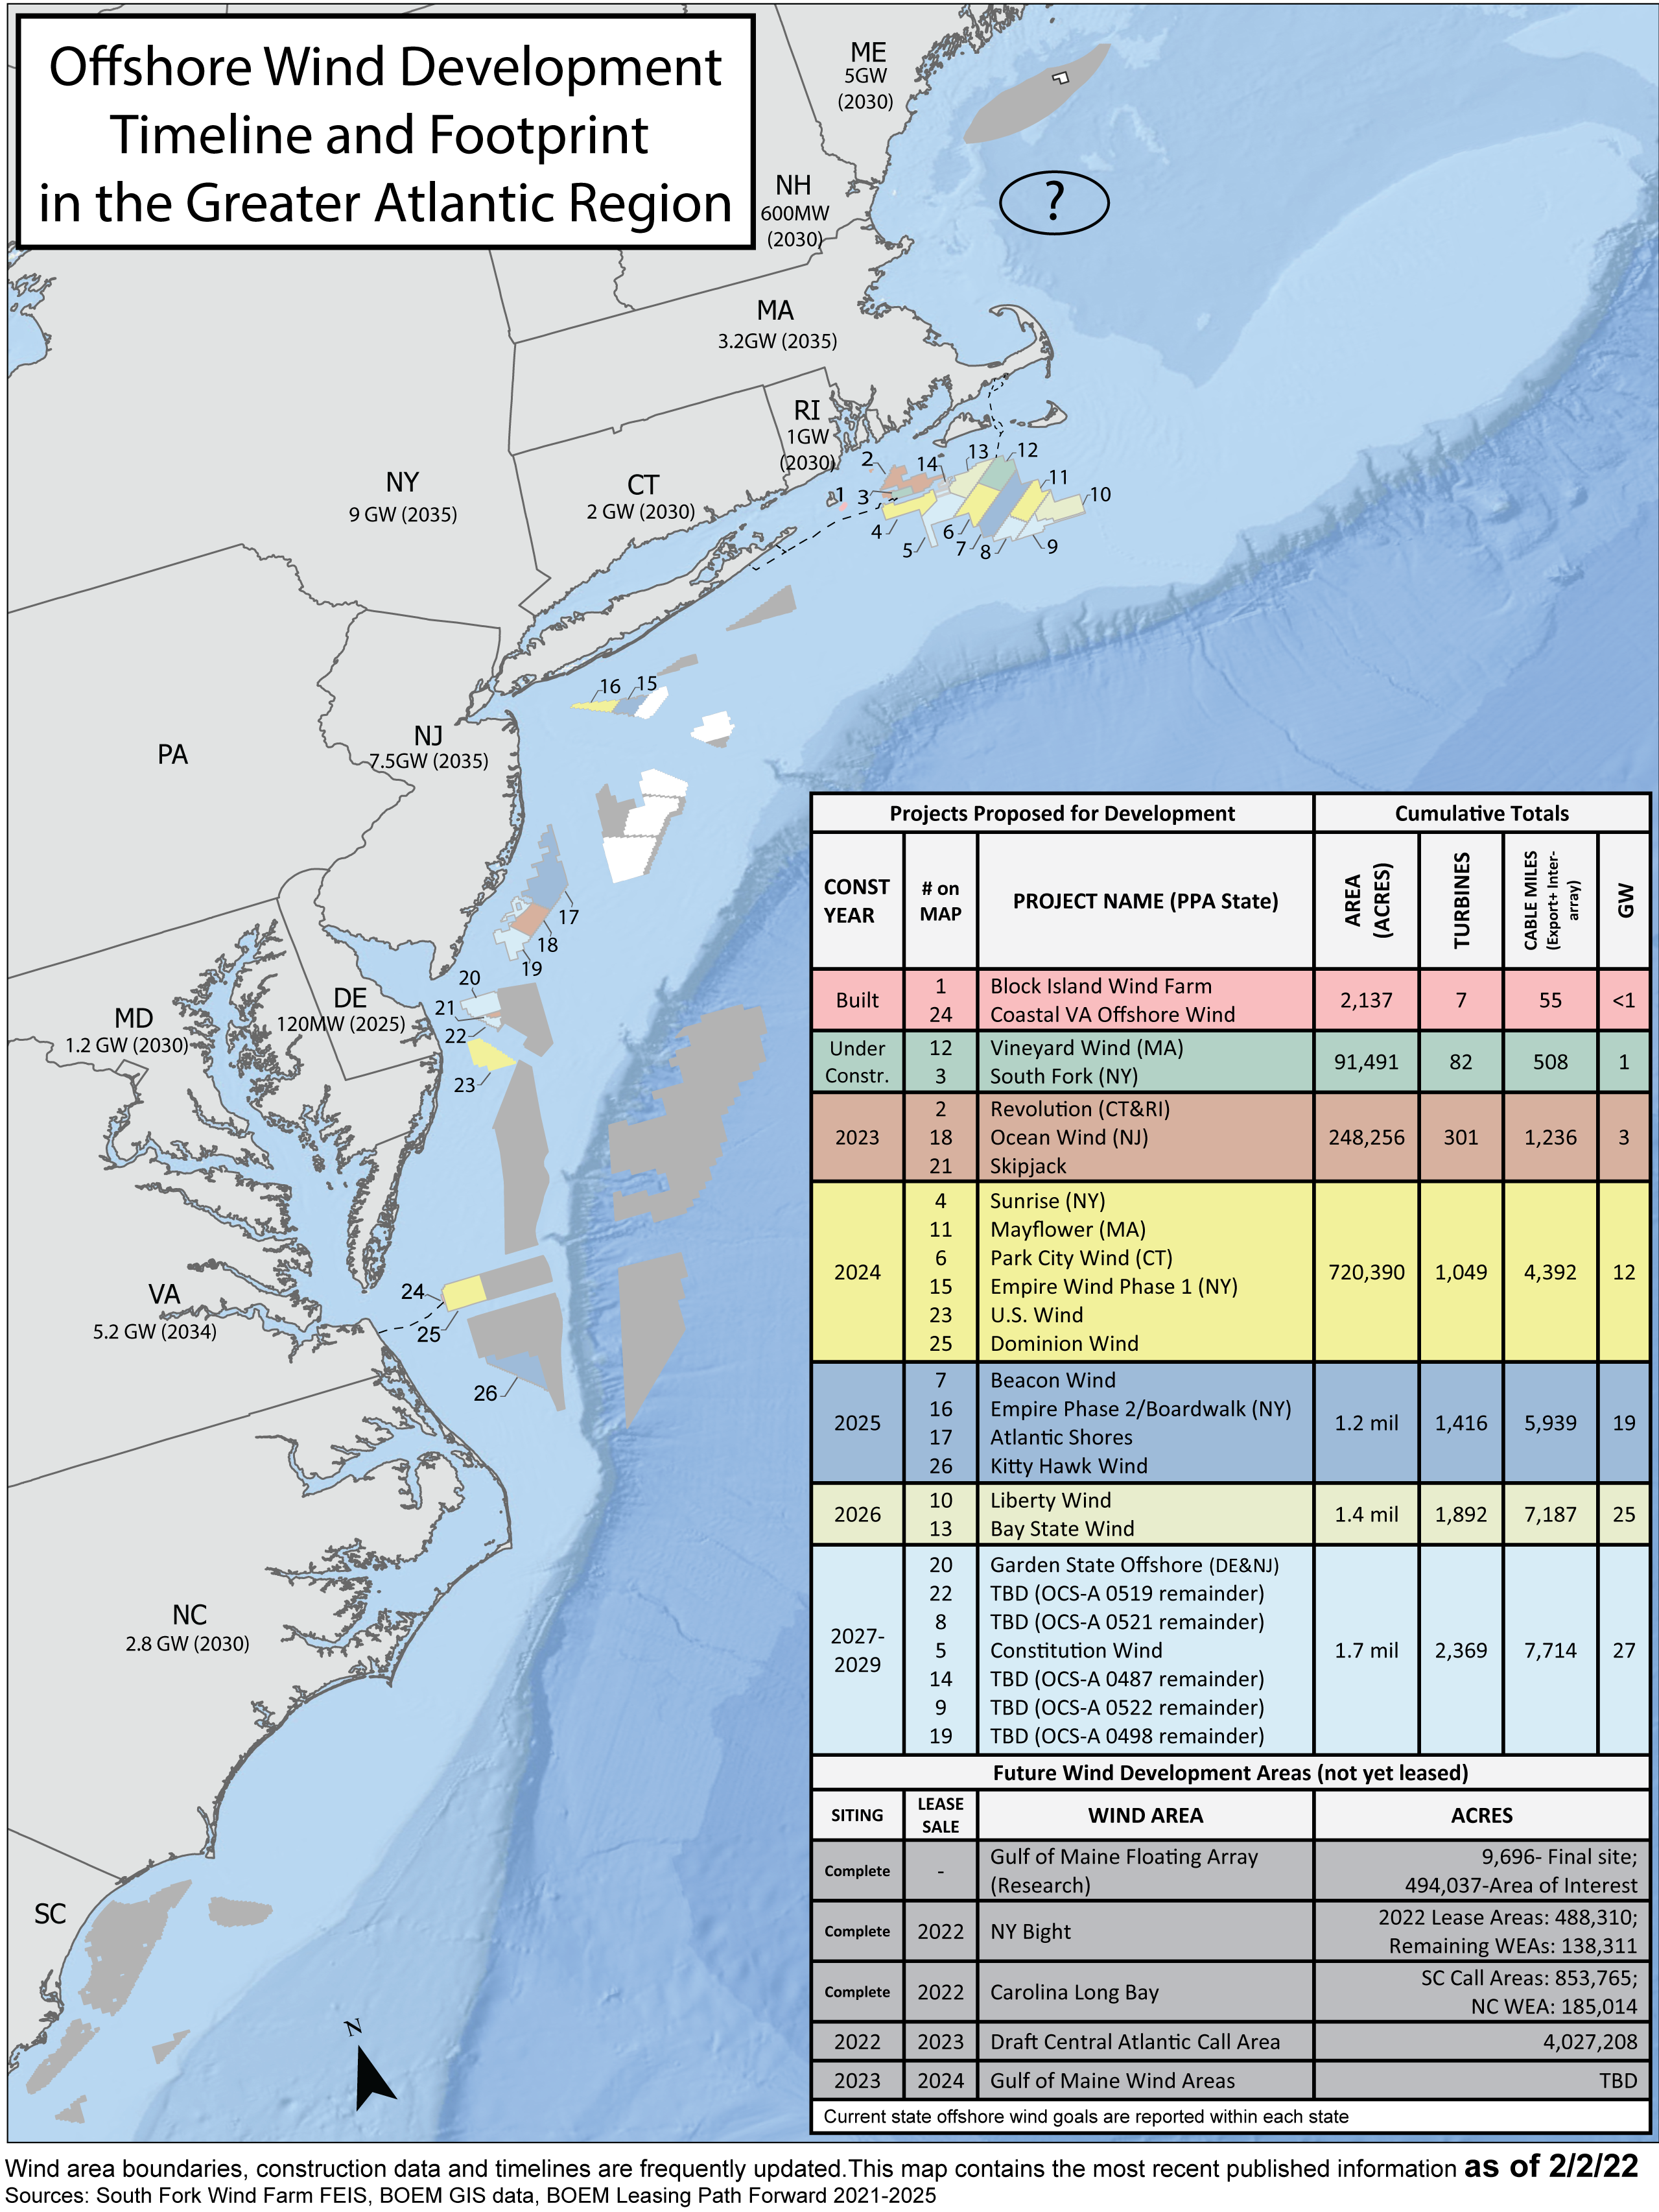
\includegraphics[width=0.9\linewidth]{images/offshore_wind_timeline} 

}

\caption{All Northeast Project areas by year construction ends (each project has 2 year construction period).}\label{fig:wind-dev-cumul}
\end{figure}

Just over 2,500 foundations and more than 7,000 miles of inter-array and
offshore export cables are proposed to date. The colored chart in Fig.
\ref{fig:wind-dev-cumul} also presents the offshore wind development
timeline in the Greater Atlantic region with the estimated year that
foundations would be constructed (matches the color of the wind areas).
These timelines and data estimates are expected to shift but represent
the most recent information available as of February 2022. Based on
current timelines, the areas affected would be spread out such that it
is unlikely that any one particular area would experience full
development at one time. Future wind development areas are also
presented. Additional lease areas, totalling over 488,000 acres in the
NY Bight are available for BOEM's 2022 lease sale. It's anticipated that
the NY Bight leases will fulfill outstanding offshore wind energy
production goals for NY and NJ. VA and NC have outstanding goals that
cannot be fulfilled within the existing lease areas, and it is expected
that these will be fulfilled with future development off the Delmarva
Peninsula.

Based on federal vessel logbook data, average commercial fishery revenue
from trips in the current offshore wind lease areas and the New York
Bight leasing areas identified in the proposed sale notice represented
2-20\% of the total annual revenue for the most affected fisheries in
federal waters from 2008-2019 (Fig. \ref{fig:wea-spp-rev}).

\begin{figure}

{\centering \includegraphics{docs/images/wea-spp-rev-1} 

}

\caption{Wind energy revenue in the Mid-Atlantic.}\label{fig:wea-spp-rev}
\end{figure}

The surfclam fishery could be the most affected fishery, with a maximum
of 20\% of annual fishery revenue occurring within potential wind lease
areas during this period, followed by chub mackerel (15\%), ocean quahog
(13\%), and Atlantic mackerel (10\%). The \emph{Illex} squid and
bluefish fisheries were the least affected, at 1-2\% maximum annual
revenue affected, respectively. A maximum of 9\% of the annual scup
revenues were affected by these areas, with similar effects for the
longfin squid (8\%), blueline tilefish and black sea bass (7\%), and
monkfish and golden tilefish (6\%) fisheries. The proposed New York
Bight lease areas represented up to 5\% of total annual fishery revenue
from any MAFMC fishery during 2008-2019, with the surfclam fishery most
affected. Similar patterns are observed when examining the proportion of
annual fishery landings within current and proposed lease areas (see
Table \ref{tab:wea-landings-rev}).

\begin{table}

\caption{\label{tab:wea-landings-rev}Top ten species Landings and Revenue from Wind Energy Areas.}
\centering
\resizebox{\linewidth}{!}{
\begin{tabular}[t]{l>{\raggedright\arraybackslash}p{10em}>{\raggedright\arraybackslash}p{10em}>{\raggedright\arraybackslash}p{10em}>{\raggedright\arraybackslash}p{10em}}
\toprule
GARFO and ASMFC Managed Species & Maximum Percent Total Annual Regional Species Landings & Minimum Percent Total Annual Regional Species Landings & Maximum Percent Total Annual Regional Species Revenue & Minimum Percent Total Annual Regional Species Revenue\\
\midrule
Atlantic surfclam & 21 \% & 6 \% & 20 \% & 6 \%\\
American eel & 13 \% & 2 \% & 18 \% & 0 \%\\
Atlantic menhaden & 17 \% & 3 \% & 17 \% & 3 \%\\
Atlantic chub mackerel & 15 \% & 0 \% & 16 \% & 0 \%\\
Yellowtail flounder & 14 \% & 0 \% & 15 \% & 0 \%\\
\addlinespace
Offshore hake & 14 \% & 0 \% & 14 \% & 0 \%\\
Ocean quahog & 14 \% & 5 \% & 13 \% & 5 \%\\
Atlantic sea scallops & 12 \% & 1 \% & 10 \% & 1 \%\\
Skate wings & 10 \% & 5 \% & 10 \% & 5 \%\\
Atlantic mackerel & 9 \% & 0 \% & 10 \% & 0 \%\\
\bottomrule
\end{tabular}}
\end{table}

Proposed wind development areas interact with the region's federal
scientific surveys. Scientific surveys are impacted by offshore wind in
four ways: 1. Exclusion of NOAA Fisheries' sampling platforms from the
wind development area due to operational and safety limitations;
2.Impacts on the random-stratified statistical design that is the basis
for scientific assessments, advice, and analyses; 3.Alteration of
benthic and pelagic habitats, and airspace in and around the wind energy
development, requiring new designs and methods to sample new habitats;
and, 4.Reduced sampling productivity through navigation impacts of wind
energy infrastructure on aerial and vessel survey operations. Increase
vessel transit between stations may decrease data collections that are
already limited by annual days-at-sea day allocations. The total survey
area overlap ranges from 1-14\% for all Greater Atlantic federal
surveys. Individual survey strata have significant interaction with
wind, including the sea scallop survey (up to 96\% of individual strata)
and the bottom trawl survey (BTS, up to 60\% strata overlap).
Additionally, up to 50\% of the southern New England North Atlantic
right whale survey's area overlaps with proposed project areas. A
region-wide survey mitigation program is underway (Table
\ref{tab:wind-survey-table})

\begin{table}

\caption{\label{tab:wind-survey-table}Survey mitigation planning.}
\centering
\resizebox{\linewidth}{!}{
\begin{tabular}[t]{l>{\raggedright\arraybackslash}p{10em}>{\raggedright\arraybackslash}p{10em}>{\raggedright\arraybackslash}p{10em}>{\raggedright\arraybackslash}p{10em}>{\raggedright\arraybackslash}p{10em}>{\raggedright\arraybackslash}p{10em}}
\toprule
Survey & 1.Evaluate designs \& Impacts & 2.Design New Methods & 3.Calibrate New/Existing Surveys & 4.Bridge Solutions & 5.Conduct New Surveys & 6.Comms \& Data\\
\midrule
Fall BTS & Started & Inital & No & No & No & Initial\\
Spring BTS & Started & Initial & No & No & No & Initial\\
EcoMon & No & No & No & No & No & No\\
Scallop & Started & Initial & No & No & No & No\\
Shellfish(Clams) & No & No & No & No & No & No\\
\addlinespace
Right Whale (Air) & Inital & Initial & Initial & No & No & No\\
Marine Mammal/Turtle (Ship/Air) & No & No & No & No & No & No\\
Altantic Shark (Bottom Long-Line & No & No & No & No & No & No\\
GOM Bottom Long-Line & No & No & No & No & No & No\\
GOM Shrimp Survey & No & No & No & No & No & No\\
\addlinespace
Atlantic Shark COASTPAN & No & No & No & No & No & No\\
\bottomrule
\end{tabular}}
\end{table}

Equity and environmental justice (EJ) are priority concerns with
offshore wind development and fisheries impacts in the Northeast. Fig.
\ref{fig:wea-port-rev} links historic port revenue (2008-2019) from
within all wind lease areas as a proportion of the port's total revenue
based on vessel trip reports as described in the revenue and landings of
species in the wind indicator above. The range (minimum and maximum) of
total percent revenue from within wind energy areas is presented in the
graph and ports are sorted from greatest to least revenue from within
wind areas.

\begin{figure}

\includegraphics{docs/images/wea-port-rev-1} \hfill{}

\caption{Percent of port revenue from Wind Energy Areas (WEA) in descending order from most to least port revenue from WEA. EJ = Environmental Justice.}\label{fig:wea-port-rev}
\end{figure}

For example, Atlantic City, NJ had a minimum of 11\% and maximum of 30\%
overlap of wind energy revenue to the total port revenue between
2008-2019. Those communities that score Med-High or higher in at least
one of the vulnerability indicators that address environmental justice
concerns (i.e., Poverty, Population Composition, Personal Disruption;
see indicator definitions) are noted with a triangle. Gentrification
pressure is also highlighted here, with those communities that score
Med-High or higher in one or more gentrification pressure indicators
(i.e., Housing Disruption, Retiree Migration, Urban Sprawl) represented
with a circle (Fig. \ref{fig:wea-port-rev}). BOEM reports that
cumulative offshore wind development (if all proposed projects are
developed) could have moderate impacts on low-income members of
environmental justice communities who work in the commercial fishing and
for-hire fishing industry due to disruptions to fish populations,
restrictions on navigation and increased vessel traffic, as well as
existing vulnerabilities of low-income workers to economic impacts
{[}\protect\hyperlink{ref-boem_vineyard_2020}{51}{]}.

Top fishing communities high in environmental justice concerns (i.e.,
Atlantic City, NJ, Newport News, VA, Hobucken and Beaufort, NC) should
be considered in decision making to reduce the social and economic
impacts and aid in the resilience and adaptive capacity of underserved
communities. It also highlights communities where we need to provide
further resources to reach underserved and underrepresented groups and
create opportunities for and directly involve these groups in the
decision-making process.

\hypertarget{implications-7}{%
\subsubsection{Implications}\label{implications-7}}

Current plans for rapid buildout of offshore wind in a patchwork of
areas spreads the impacts differentially throughout the region (Fig.
\ref{fig:wind-dev-cumul}).

Up to 20\% of total average revenue for major Mid-Atlantic commercial
species in lease areas could be forgone or reduced and associated effort
displaced if all sites are developed. Displaced fishing effort can alter
historic fishing area, timing, and method patterns, which can in turn
change habitat, species (managed and protected), and fleet interactions.
Several factors, including fishery regulations, fishery availability,
and user conflicts affect where, when, and how fishing effort may be
displaced.

Planned development overlaps right whale mother and calf migration
corridors and a significant foraging habitat that is used throughout the
year {[}\protect\hyperlink{ref-quintana-rizzo_residency_2021}{9}{]} (Fig
\ref{fig:whales-wind}). Turbine presence and extraction of energy from
the system could alter local oceanography
{[}\protect\hyperlink{ref-christiansen_emergence_2022}{52}{]} and may
affect right whale prey availability. Proposed wind development areas
also bring increased vessel strike risk from construction and operation
vessels. In addition, there are a number of potential impacts to whales
from pile driving and operational noise such as displacement, increased
levels of communication masking, and elevated stress hormones.

\begin{figure}

{\centering 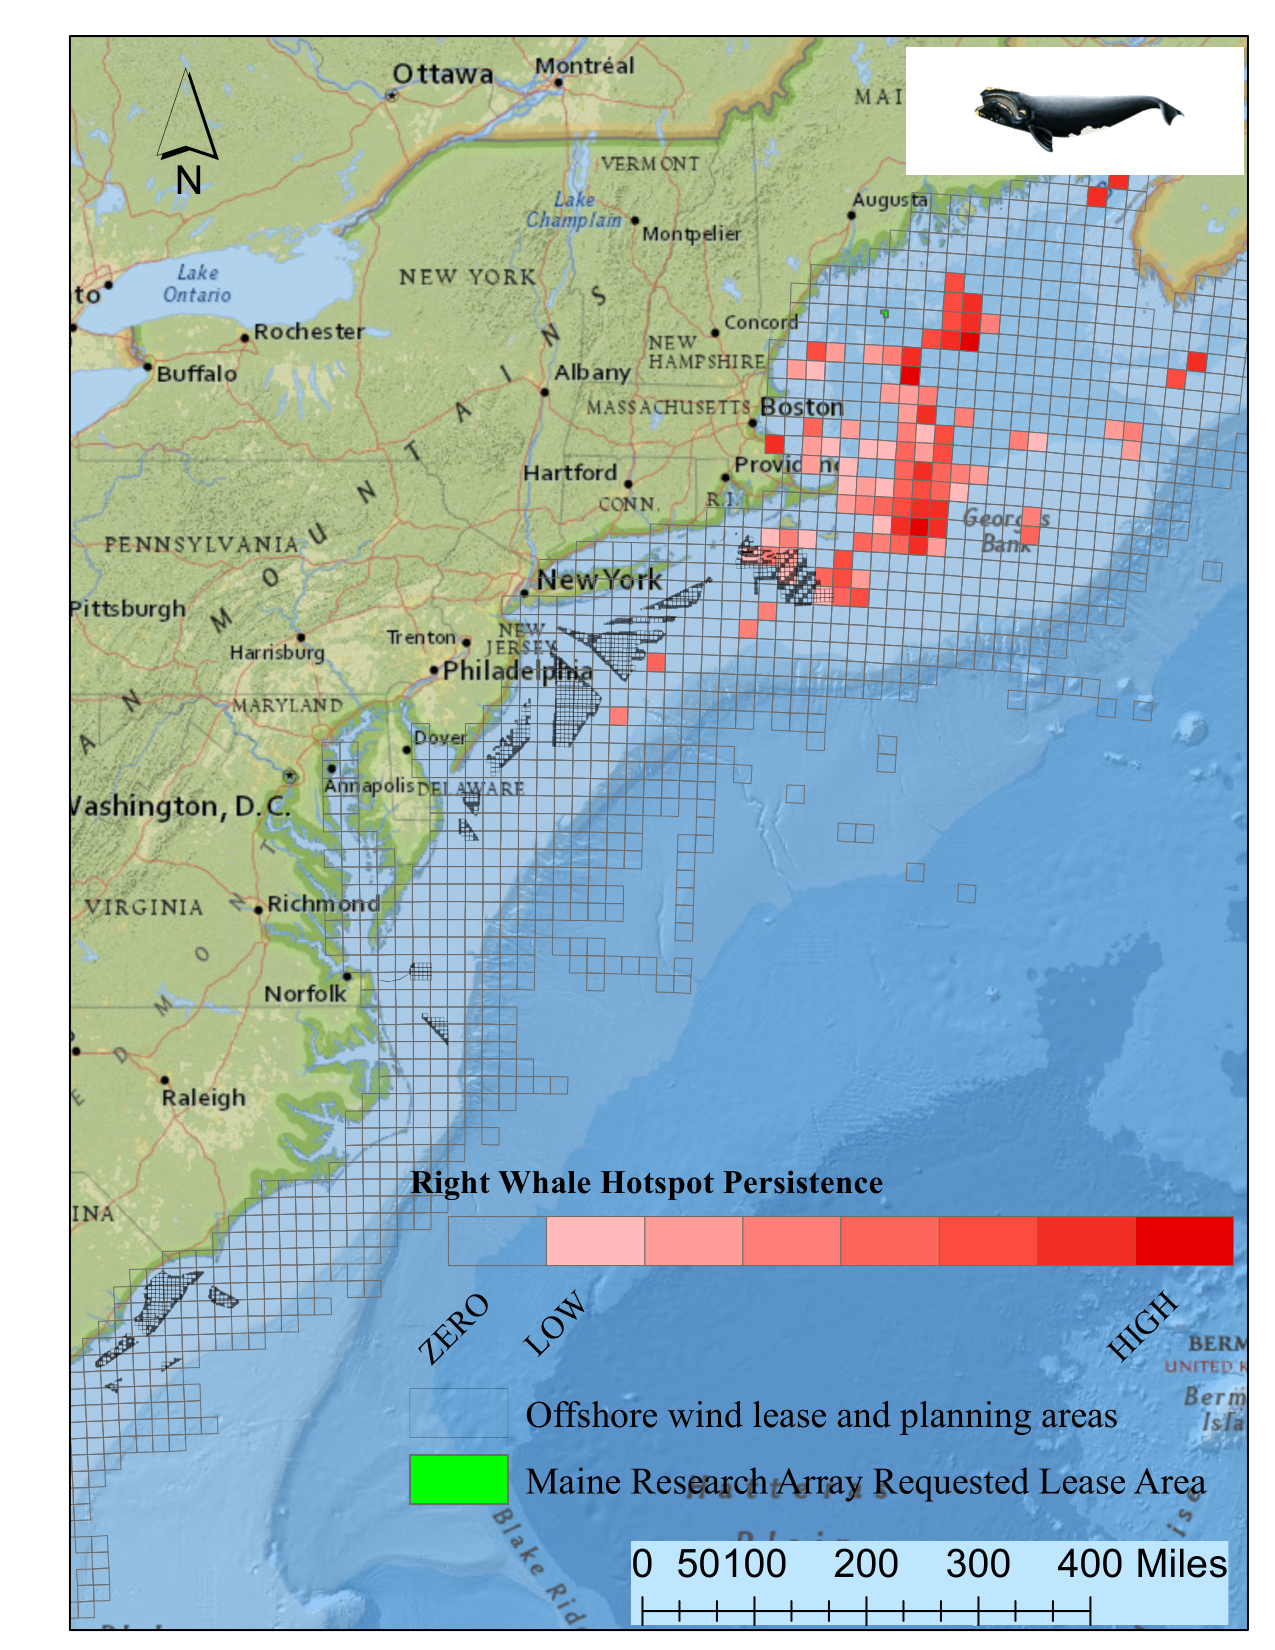
\includegraphics[width=0.6\linewidth]{images/NARW_hotpsot_persistence_2_1_2022_TPW} 

}

\caption{Northern Right Whale persistent hotspots and Wind Energy Areas.}\label{fig:whales-wind}
\end{figure}

Scientific data collection surveys for ocean and ecosystem conditions,
fish, and protected species will be altered, potentially increasing
uncertainty for management decision making.

The increase of offshore wind development can have both positive (e.g.,
employment opportunities) and negative (e.g., space-use conflicts)
effects. Continued increase in coastal development and gentrification
pressure has resulted in loss of fishing infrastructure space within
ports. Understanding these existing pressures can allow for avoiding and
mitigating negative impacts to our shore support industry and
communities dependent on fishing. Some of the communities with the
highest revenue overlap with offshore wind that are also vulnerable to
gentrification pressure are Point Pleasant and Atlantic City, NJ, Ocean
City, MD, and Beaufort, NC.

\hypertarget{contributors}{%
\section{Contributors}\label{contributors}}

\textbf{Editors} (NOAA NMFS Northeast Fisheries Science Center, NEFSC):
Sarah Gaichas, Kimberly Bastille, Geret DePiper, Kimberly Hyde, Scott
Large, Sean Lucey, Chris Orphanides, Laurel Smith

\textbf{Contributors} (NEFSC unless otherwise noted): Kimberly Bastille,
Aaron Beaver (Anchor QEA), Andy Beet, Ruth Boettcher (Virginia
Department of Game and Inland Fisheries), Mandy Bromilow and CJ Pellerin
(NOAA Chesapeake Bay Office), Joseph Caracappa, Doug Christel (GARFO),
Patricia Clay, Lisa Colburn, Jennifer Cudney and Tobey Curtis (NMFS
Atlantic HMS Management Division), Geret DePiper, Dan Dorfman
(NOAA-NOS-NCCOS), Hubert du Pontavice, Emily Farr and Grace Roskar (NMFS
Office of Habitat Conservation), Michael Fogarty, Paula Fratantoni,
Kevin Friedland, Marjy Friedrichs (VIMS), Sarah Gaichas, Ben Galuardi
(GAFRO), Avijit Gangopadhyay (School for Marine Science and Technology,
University of Massachusetts Dartmouth), James Gartland (Virginia
Institute of Marine Science), Glen Gawarkiewicz (Woods Hole
Oceanographic Institution), Sean Hardison, Kimberly Hyde, John Kosik,
Steve Kress and Don Lyons (National Audubon Society's Seabird
Restoration Program), Young-Oh Kwon and Zhuomin Chen (Woods Hole
Oceanographic Institution), Andrew Lipsky, Sean Lucey, Chris Melrose,
Shannon Meseck, Ryan Morse, Brandon Muffley (MAFMC), Kimberly Murray,
Chris Orphanides, Richard Pace, Tom Parham (Maryland DNR), Charles
Perretti, Grace Saba and Emily Slesinger (Rutgers University), Vincent
Saba, Sarah Salois, Chris Schillaci (GARFO), Dave Secor (CBL), Angela
Silva, Adrienne Silver (UMass/SMAST), Laurel Smith, Talya ten Brink
(GARFO), Bruce Vogt (NOAA Chesapeake Bay Office), Ron Vogel (University
of Maryland Cooperative Institute for Satellite Earth System Studies and
NOAA/NESDIS Center for Satellite Applications and Research), John
Walden, Harvey Walsh, Changhua Weng, Mark Wuenschel

\newpage

\hypertarget{document-orientation}{%
\section{Document Orientation}\label{document-orientation}}

The figure format is illustrated in Fig \ref{fig:docformat}a. Trend
lines are shown when slope is significantly different from 0 at the p
\textless{} 0.05 level. An orange line signifies an overall positive
trend, and purple signifies a negative trend. To minimize bias
introduced by small sample size, no trend is fit for \textless{} 30 year
time series. Dashed lines represent mean values of time series unless
the indicator is an anomaly, in which case the dashed line is equal to
0. Shaded regions indicate the past ten years. If there are no new data
for 2021, the shaded region will still cover this time period. The
spatial scale of indicators is either coastwide, Mid-Atlantic states
(New York, New Jersey, Delaware, Maryland, Virginia, North Carolina), or
at the Mid-Atlantic Bight (MAB) Ecosystem Production Unit (EPU, Fig.
\ref{fig:docformat}b) level.

\begin{figure}

{\centering \includegraphics{docs/images/docformat-1} 

}

\caption{Document orientation. a. Key to figures. b.The Northeast Large Marine Ecosystem.}\label{fig:docformat}
\end{figure}

Fish and invertebrates are aggregated into similar feeding categories
(Table \ref{tab:species-groupings}) to evaluate ecosystem level trends
in predators and prey.

\begin{table}[!h]

\caption{\label{tab:species-groupings}Feeding guilds and management bodies.}
\centering
\resizebox{\linewidth}{!}{
\fontsize{10}{12}\selectfont
\begin{tabular}[t]{>{\raggedright\arraybackslash}p{2cm}>{\raggedright\arraybackslash}p{4cm}>{\raggedright\arraybackslash}p{2cm}>{\raggedright\arraybackslash}p{5cm}>{\raggedright\arraybackslash}p{6cm}}
\toprule
\textbf{Guild} & \textbf{MAFMC} & \textbf{Joint} & \textbf{NEFMC} & \textbf{State or Other}\\
\midrule
Apex Predator & NA & NA & NA & bluefin tuna, shark uncl, swordfish, yellowfin tuna\\
\cmidrule{1-5}
Piscivore & bluefish, longfin squid, northern shortfin squid, summer flounder & goosefish, spiny dogfish & acadian redfish, atlantic cod, atlantic halibut, clearnose skate, little skate, offshore hake, pollock, red hake, silver hake, smooth skate, thorny skate, white hake, winter skate & fourspot flounder, john dory, sea raven, striped bass, weakfish, windowpane\\
\cmidrule{1-5}
Planktivore & atlantic mackerel, butterfish & NA & atlantic herring & alewife, american shad, blackbelly rosefish, blueback herring, cusk, longhorn sculpin, lumpfish, menhaden, northern sand lance, northern searobin, sculpin uncl\\
\cmidrule{1-5}
Benthivore & black sea bass, scup, tilefish & NA & american plaice, barndoor skate, crab,red deepsea, haddock, ocean pout, rosette skate, winter flounder, witch flounder, yellowtail flounder & american lobster, atlantic wolffish, blue crab, cancer crab uncl, chain dogfish, cunner, jonah crab, lady crab, smooth dogfish, spider crab uncl, squid cuttlefish and octopod uncl, striped searobin, tautog\\
\cmidrule{1-5}
Benthos & atlantic surfclam, ocean quahog & NA & sea scallop & blue mussel, channeled whelk, sea cucumber, sea urchin and sand dollar uncl, sea urchins, snails(conchs)\\
\bottomrule
\end{tabular}}
\end{table}

\newpage

\hypertarget{references}{%
\section*{References}\label{references}}
\addcontentsline{toc}{section}{References}

\hypertarget{refs}{}
\begin{CSLReferences}{0}{0}
\leavevmode\hypertarget{ref-thunberg_northeast_2021}{}%
\CSLLeftMargin{1. }
\CSLRightInline{Thunberg EM. Northeast {Region} {Fisheries} {Impacts}
from {COVID}-19. U{S} {Seafood} {Industry} and {For}-{Hire} {Sector}
{Impacts} from {COVID}-19: 2020 in {Perspective} {NOAA} {Tech} {Memo}
{NMFS}-{SPO}-221. 2021. pp. 53--64. Available:
\url{https://spo.nmfs.noaa.gov/sites/default/files/TM221.pdf}}

\leavevmode\hypertarget{ref-gaichas_implementing_2018}{}%
\CSLLeftMargin{2. }
\CSLRightInline{Gaichas SK, DePiper GS, Seagraves RJ, Muffley BW, Sabo
M, Colburn LL, et al. Implementing {Ecosystem} {Approaches} to {Fishery}
{Management}: {Risk} {Assessment} in the {US} {Mid}-{Atlantic}.
Frontiers in Marine Science. 2018;5.
doi:\href{https://doi.org/10.3389/fmars.2018.00442}{10.3389/fmars.2018.00442}}

\leavevmode\hypertarget{ref-friedland_changes_2020}{}%
\CSLLeftMargin{3. }
\CSLRightInline{Friedland KD, Langan JA, Large SI, Selden RL, Link JS,
Watson RA, et al. Changes in higher trophic level productivity,
diversity and niche space in a rapidly warming continental shelf
ecosystem. Science of The Total Environment. 2020;704: 135270.
doi:\href{https://doi.org/10.1016/j.scitotenv.2019.135270}{10.1016/j.scitotenv.2019.135270}}

\leavevmode\hypertarget{ref-pace_cryptic_2021}{}%
\CSLLeftMargin{4. }
\CSLRightInline{Pace RM, Williams R, Kraus SD, Knowlton AR, Pettis HM.
Cryptic mortality of {North} {Atlantic} right whales. Conservation
Science and Practice. 2021;n/a: e346.
doi:\url{https://doi.org/10.1111/csp2.346}}

\leavevmode\hypertarget{ref-wood_rates_2020}{}%
\CSLLeftMargin{5. }
\CSLRightInline{Wood SA, Murray KT, Josephson E, Gilbert J. Rates of
increase in gray seal ({Halichoerus} grypus atlantica) pupping at
recolonized sites in the {United} {States}, 1988--2019. Swanson B,
editor. Journal of Mammalogy. 2020;101: 121--128.
doi:\href{https://doi.org/10.1093/jmammal/gyz184}{10.1093/jmammal/gyz184}}

\leavevmode\hypertarget{ref-hayes_north_2018}{}%
\CSLLeftMargin{6. }
\CSLRightInline{Hayes S, Gardner S, Garrison LP, Henry A, Leandro L.
North {Atlantic} {Right} {Whales}-{Evaluating} {Their} {Recovery}
{Challenges} in 2018. {NOAA} {Tech} {Memo} {NMFS} {NEFSC} 247. 2018. }

\leavevmode\hypertarget{ref-record_rapid_2019}{}%
\CSLLeftMargin{7. }
\CSLRightInline{Record N, Runge J, Pendleton D, Balch W, Davies K,
Pershing A, et al. Rapid {Climate}-{Driven} {Circulation} {Changes}
{Threaten} {Conservation} of {Endangered} {North} {Atlantic} {Right}
{Whales}. Oceanography. 2019;32.
doi:\href{https://doi.org/10.5670/oceanog.2019.201}{10.5670/oceanog.2019.201}}

\leavevmode\hypertarget{ref-sorochan_north_2019}{}%
\CSLLeftMargin{8. }
\CSLRightInline{Sorochan KA, Plourde S, Morse R, Pepin P, Runge J,
Thompson C, et al. North {Atlantic} right whale ({Eubalaena} glacialis)
and its food: ({II}) interannual variations in biomass of {Calanus} spp.
On western {North} {Atlantic} shelves. Journal of Plankton Research.
2019;41: 687--708.
doi:\href{https://doi.org/10.1093/plankt/fbz044}{10.1093/plankt/fbz044}}

\leavevmode\hypertarget{ref-quintana-rizzo_residency_2021}{}%
\CSLLeftMargin{9. }
\CSLRightInline{Quintana-Rizzo E, Leiter S, Cole TVN, Hagbloom MN,
Knowlton AR, Nagelkirk P, et al. Residency, demographics, and movement
patterns of {North} {Atlantic} right whales {Eubalaena} glacialis in an
offshore wind energy development area in southern {New} {England},
{USA}. Endangered Species Research. 2021;45: 251--268.
doi:\href{https://doi.org/10.3354/esr01137}{10.3354/esr01137}}

\leavevmode\hypertarget{ref-schick_striking_2009}{}%
\CSLLeftMargin{10. }
\CSLRightInline{Schick RS, Halpin PN, Read AJ, Slay CK, Kraus SD, Mate
BR, et al. Striking the right balance in right whale conservation.
Canadian Journal of Fisheries and Aquatic Sciences. 2009;66: 1399--1403.
doi:\href{https://doi.org/10.1139/F09-115}{10.1139/F09-115}}

\leavevmode\hypertarget{ref-hobday_hierarchical_2016}{}%
\CSLLeftMargin{11. }
\CSLRightInline{Hobday AJ, Alexander LV, Perkins SE, Smale DA, Straub
SC, Oliver ECJ, et al. A hierarchical approach to defining marine
heatwaves. Progress in Oceanography. 2016;141: 227--238.
doi:\href{https://doi.org/10.1016/j.pocean.2015.12.014}{10.1016/j.pocean.2015.12.014}}

\leavevmode\hypertarget{ref-gangopadhyay_census_2020}{}%
\CSLLeftMargin{12. }
\CSLRightInline{Gangopadhyay A, Gawarkiewicz G, Silva ENS, Silver AM,
Monim M, Clark J. A {Census} of the {Warm}-{Core} {Rings} of the {Gulf}
{Stream}: 1980--2017. Journal of Geophysical Research: Oceans. 2020;125:
e2019JC016033.
doi:\href{https://doi.org/10.1029/2019JC016033}{10.1029/2019JC016033}}

\leavevmode\hypertarget{ref-andres_recent_2016}{}%
\CSLLeftMargin{13. }
\CSLRightInline{Andres M. On the recent destabilization of the {Gulf}
{Stream} path downstream of {Cape} {Hatteras}. Geophysical Research
Letters. 2016;43: 9836--9842.
doi:\href{https://doi.org/10.1002/2016GL069966}{10.1002/2016GL069966}}

\leavevmode\hypertarget{ref-caesar_observed_2018}{}%
\CSLLeftMargin{14. }
\CSLRightInline{Caesar L, Rahmstorf S, Robinson A, Feulner G, Saba V.
Observed fingerprint of a weakening {Atlantic} {Ocean} overturning
circulation. Nature. 2018;556: 191--196.
doi:\href{https://doi.org/10.1038/s41586-018-0006-5}{10.1038/s41586-018-0006-5}}

\leavevmode\hypertarget{ref-zhang_role_2007}{}%
\CSLLeftMargin{15. }
\CSLRightInline{Zhang R, Vallis GK. The {Role} of {Bottom} {Vortex}
{Stretching} on the {Path} of the {North} {Atlantic} {Western}
{Boundary} {Current} and on the {Northern} {Recirculation} {Gyre}.
Journal of Physical Oceanography. 2007;37: 2053--2080.
doi:\href{https://doi.org/10.1175/JPO3102.1}{10.1175/JPO3102.1}}

\leavevmode\hypertarget{ref-goddard_extreme_2015}{}%
\CSLLeftMargin{16. }
\CSLRightInline{Goddard PB, Yin J, Griffies SM, Zhang S. An extreme
event of sea-level rise along the {Northeast} coast of {North} {America}
in 2009--2010. Nature Communications. 2015;6.
doi:\href{https://doi.org/10.1038/ncomms7346}{10.1038/ncomms7346}}

\leavevmode\hypertarget{ref-goncalves_neto_changes_2021}{}%
\CSLLeftMargin{17. }
\CSLRightInline{Gonçalves Neto A, Langan JA, Palter JB. Changes in the
{Gulf} {Stream} preceded rapid warming of the {Northwest} {Atlantic}
{Shelf}. Communications Earth \& Environment. 2021;2: 1--10.
doi:\href{https://doi.org/10.1038/s43247-021-00143-5}{10.1038/s43247-021-00143-5}}

\leavevmode\hypertarget{ref-silver_forecasting_2021}{}%
\CSLLeftMargin{18. }
\CSLRightInline{Silver A, Gangopadhyay A, Gawarkiewicz G, Taylor A,
Sanchez-Franks A. Forecasting the {Gulf} {Stream} {Path} {Using}
{Buoyancy} and {Wind} {Forcing} {Over} the {North} {Atlantic}. Journal
of Geophysical Research: Oceans. 2021;126: e2021JC017614.
doi:\href{https://doi.org/10.1029/2021JC017614}{10.1029/2021JC017614}}

\leavevmode\hypertarget{ref-gangopadhyay_observed_2019}{}%
\CSLLeftMargin{19. }
\CSLRightInline{Gangopadhyay A, Gawarkiewicz G, Silva ENS, Monim M,
Clark J. An {Observed} {Regime} {Shift} in the {Formation} of {Warm}
{Core} {Rings} from the {Gulf} {Stream}. Scientific Reports. 2019;9:
1--9.
doi:\href{https://doi.org/10.1038/s41598-019-48661-9}{10.1038/s41598-019-48661-9}}

\leavevmode\hypertarget{ref-gawarkiewicz_changing_2018}{}%
\CSLLeftMargin{20. }
\CSLRightInline{Gawarkiewicz G, Todd R, Zhang W, Partida J, Gangopadhyay
A, Monim M-U-H, et al. The {Changing} {Nature} of {Shelf}-{Break}
{Exchange} {Revealed} by the {OOI} {Pioneer} {Array}. Oceanography.
2018;31: 60--70.
doi:\href{https://doi.org/10.5670/oceanog.2018.110}{10.5670/oceanog.2018.110}}

\leavevmode\hypertarget{ref-chen_mesoscale_2022}{}%
\CSLLeftMargin{21. }
\CSLRightInline{Chen K, Gawarkiewicz G, Yang J. Mesoscale and
{Submesoscale} {Shelf}-{Ocean} {Exchanges} {Initialize} an {Advective}
{Marine} {Heatwave}. Journal of Geophysical Research: Oceans. 2022;127:
e2021JC017927. doi:\url{https://doi.org/10.1029/2021JC017927}}

\leavevmode\hypertarget{ref-gawarkiewicz_increasing_nodate}{}%
\CSLLeftMargin{22. }
\CSLRightInline{Gawarkiewicz G, Fratantoni P, Bahr F, Ellertson A.
Increasing {Frequency} of {Mid}-depth {Salinity} {Maximum} {Intrusions}
in the {Middle} {Atlantic} {Bight}. Journal of Geophysical Research:
Oceans. In Review; }

\leavevmode\hypertarget{ref-gawarkiewicz_characteristics_2019}{}%
\CSLLeftMargin{23. }
\CSLRightInline{Gawarkiewicz G, Chen K, Forsyth J, Bahr F, Mercer AM,
Ellertson A, et al. Characteristics of an {Advective} {Marine}
{Heatwave} in the {Middle} {Atlantic} {Bight} in {Early} 2017. Frontiers
in Marine Science. 2019;6. Available:
\url{https://www.frontiersin.org/article/10.3389/fmars.2019.00712}}

\leavevmode\hypertarget{ref-potter_horizontal_2011}{}%
\CSLLeftMargin{24. }
\CSLRightInline{Potter IF, Galuardi B, Howell WH. Horizontal movement of
ocean sunfish, {Mola} mola, in the northwest {Atlantic}. Marine Biology.
2011;158: 531--540.
doi:\href{https://doi.org/10.1007/s00227-010-1578-2}{10.1007/s00227-010-1578-2}}

\leavevmode\hypertarget{ref-worm_predator_2003}{}%
\CSLLeftMargin{25. }
\CSLRightInline{Worm B, Lotze HK, Myers RA. Predator diversity hotspots
in the blue ocean. Proceedings of the National Academy of Sciences.
2003;100: 9884--9888.
doi:\href{https://doi.org/10.1073/pnas.1333941100}{10.1073/pnas.1333941100}}

\leavevmode\hypertarget{ref-lentz_seasonal_2017}{}%
\CSLLeftMargin{26. }
\CSLRightInline{Lentz SJ. Seasonal warming of the {Middle} {Atlantic}
{Bight} {Cold} {Pool}. Journal of Geophysical Research: Oceans.
2017;122: 941--954.
doi:\href{https://doi.org/10.1002/2016JC012201}{10.1002/2016JC012201}}

\leavevmode\hypertarget{ref-chen_seasonal_2018}{}%
\CSLLeftMargin{27. }
\CSLRightInline{Chen Z, Curchitser E, Chant R, Kang D. Seasonal
{Variability} of the {Cold} {Pool} {Over} the {Mid}-{Atlantic} {Bight}
{Continental} {Shelf}. Journal of Geophysical Research: Oceans.
2018;123: 8203--8226.
doi:\href{https://doi.org/10.1029/2018JC014148}{10.1029/2018JC014148}}

\leavevmode\hypertarget{ref-miles_offshore_2021}{}%
\CSLLeftMargin{28. }
\CSLRightInline{Miles T, Murphy S, Kohut J, Borsetti S, Munroe D.
Offshore {Wind} {Energy} and the {Mid}-{Atlantic} {Cold} {Pool}: {A}
{Review} of {Potential} {Interactions}. Marine Technology Society
Journal. 2021;55: 72--87.
doi:\href{https://doi.org/10.4031/MTSJ.55.4.8}{10.4031/MTSJ.55.4.8}}

\leavevmode\hypertarget{ref-miller_state-space_2016}{}%
\CSLLeftMargin{29. }
\CSLRightInline{Miller TJ, Hare JA, Alade LA. A state-space approach to
incorporating environmental effects on recruitment in an age-structured
assessment model with an application to southern {New} {England}
yellowtail flounder. Canadian Journal of Fisheries and Aquatic Sciences.
2016;73: 1261--1270.
doi:\href{https://doi.org/10.1139/cjfas-2015-0339}{10.1139/cjfas-2015-0339}}

\leavevmode\hypertarget{ref-du_pontavice_incorporating_nodate}{}%
\CSLLeftMargin{30. }
\CSLRightInline{Pontavice H du, Miller TJ, Stock BC, Chen Z, Saba VS.
Incorporating environmental effects from ocean models improves a marine
fish stock assessment. ICES Journal of Marine Science. In Review; }

\leavevmode\hypertarget{ref-friedland_middle_2022}{}%
\CSLLeftMargin{31. }
\CSLRightInline{Friedland KD, Miles T, Goode AG, Powell EN, Brady DC.
The {Middle} {Atlantic} {Bight} {Cold} {Pool} is warming and shrinking:
{Indices} from in situ autumn seafloor temperatures. Fisheries
Oceanography. 2022;31: 217--223.
doi:\href{https://doi.org/10.1111/fog.12573}{10.1111/fog.12573}}

\leavevmode\hypertarget{ref-wrightfairbanks_autonomous_2020}{}%
\CSLLeftMargin{32. }
\CSLRightInline{Wright‐Fairbanks EK, Miles TN, Cai W-J, Chen B, Saba GK.
Autonomous {Observation} of {Seasonal} {Carbonate} {Chemistry}
{Dynamics} in the {Mid}-{Atlantic} {Bight}. Journal of Geophysical
Research: Oceans. 2020;125: e2020JC016505.
doi:\url{https://doi.org/10.1029/2020JC016505}}

\leavevmode\hypertarget{ref-madin_periodic_2006}{}%
\CSLLeftMargin{33. }
\CSLRightInline{Madin LP, Kremer P, Wiebe PH, Purcell JE, Horgan EH,
Nemazie DA. Periodic swarms of the salp {Salpa} aspera in the {Slope}
{Water} off the {NE} {United} {States}: {Biovolume}, vertical migration,
grazing, and vertical flux. Deep Sea Research Part I: Oceanographic
Research Papers. 2006;53: 804--819.
doi:\href{https://doi.org/10.1016/j.dsr.2005.12.018}{10.1016/j.dsr.2005.12.018}}

\leavevmode\hypertarget{ref-deibel_predictability_2009}{}%
\CSLLeftMargin{34. }
\CSLRightInline{Deibel D, Paffenhofer G-A. Predictability of patches of
neritic salps and doliolids ({Tunicata}, {Thaliacea}). Journal of
Plankton Research. 2009;31: 1571--1579.
doi:\href{https://doi.org/10.1093/plankt/fbp091}{10.1093/plankt/fbp091}}

\leavevmode\hypertarget{ref-steimle_energy_1985}{}%
\CSLLeftMargin{35. }
\CSLRightInline{Steimle F, Terranova R. Energy {Equivalents} of {Marine}
{Organisms} from the {Continental} {Shelf} of the {Temperate}
{Northwest} {Atlantic}. Journal of Northwest Atlantic Fishery Science.
1985;6. doi:\href{https://doi.org/10.2960/J.v6.a11}{10.2960/J.v6.a11}}

\leavevmode\hypertarget{ref-lawson_important_1998}{}%
\CSLLeftMargin{36. }
\CSLRightInline{Lawson JW, Magalhães AM, Miller EH. Important prey
species of marine vertebrate predators in the northwest {Atlantic}:
Proximate composition and energy density. Marine Ecology Progress
Series. 1998;164: 13--20. Available:
\url{https://www.jstor.org/stable/24825521}}

\leavevmode\hypertarget{ref-le_cren_length-weight_1951}{}%
\CSLLeftMargin{37. }
\CSLRightInline{Le Cren ED. The {Length}-{Weight} {Relationship} and
{Seasonal} {Cycle} in {Gonad} {Weight} and {Condition} in the {Perch}
({Perca} fluviatilis). Journal of Animal Ecology. 1951;20: 201--219.
doi:\href{https://doi.org/10.2307/1540}{10.2307/1540}}

\leavevmode\hypertarget{ref-farr_assessment_2021}{}%
\CSLLeftMargin{38. }
\CSLRightInline{Farr ER, Johnson MR, Nelson MW, Hare JA, Morrison WE,
Lettrich MD, et al. An assessment of marine, estuarine, and riverine
habitat vulnerability to climate change in the {Northeast} {U}.{S}. PLOS
ONE. 2021;16: e0260654.
doi:\href{https://doi.org/10.1371/journal.pone.0260654}{10.1371/journal.pone.0260654}}

\leavevmode\hypertarget{ref-hare_vulnerability_2016}{}%
\CSLLeftMargin{39. }
\CSLRightInline{Hare JA, Morrison WE, Nelson MW, Stachura MM, Teeters
EJ, Griffis RB, et al. A {Vulnerability} {Assessment} of {Fish} and
{Invertebrates} to {Climate} {Change} on the {Northeast} {U}.{S}.
{Continental} {Shelf}. PLOS ONE. 2016;11: e0146756.
doi:\href{https://doi.org/10.1371/journal.pone.0146756}{10.1371/journal.pone.0146756}}

\leavevmode\hypertarget{ref-zhang_chesapeake_2018}{}%
\CSLLeftMargin{40. }
\CSLRightInline{Zhang Q, Murphy RR, Tian R, Forsyth MK, Trentacoste EM,
Keisman J, et al. Chesapeake {Bay}'s water quality condition has been
recovering: {Insights} from a multimetric indicator assessment of thirty
years of tidal monitoring data. Science of The Total Environment.
2018;637-638: 1617--1625.
doi:\href{https://doi.org/10.1016/j.scitotenv.2018.05.025}{10.1016/j.scitotenv.2018.05.025}}

\leavevmode\hypertarget{ref-bauer_temperature-_2010}{}%
\CSLLeftMargin{41. }
\CSLRightInline{Bauer LJ, Miller TJ. Temperature-, {Salinity}-, and
{Size}-{Dependent} {Winter} {Mortality} of {Juvenile} {Blue} {Crabs} (
{Callinectes} sapidus ). Estuaries and Coasts. 2010;33: 668--677.
Available: \url{https://www.jstor.org/stable/40663676}}

\leavevmode\hypertarget{ref-hines_predicting_2011}{}%
\CSLLeftMargin{42. }
\CSLRightInline{Hines AH, Johnson EG, Darnell MZ, Rittschof D, Miller
TJ, Bauer LJ, et al. Predicting {Effects} of {Climate} {Change} on
{Blue} {Crabs} in {Chesapeake} {Bay}. Biology and {Management} of
{Exploited} {Crab} {Populations} under {Climate} {Change}. Alaska Sea
Grant, University of Alaska Fairbanks; 2011. pp. 109--127.
doi:\href{https://doi.org/10.4027/bmecpcc.2010.22}{10.4027/bmecpcc.2010.22}}

\leavevmode\hypertarget{ref-rome_linking_2005}{}%
\CSLLeftMargin{43. }
\CSLRightInline{Rome MS, Young-Williams AC, Davis GR, Hines AH. Linking
temperature and salinity tolerance to winter mortality of {Chesapeake}
{Bay} blue crabs ({Callinectes} sapidus). Journal of Experimental Marine
Biology and Ecology. 2005;319: 129--145.
doi:\href{https://doi.org/10.1016/j.jembe.2004.06.014}{10.1016/j.jembe.2004.06.014}}

\leavevmode\hypertarget{ref-johnson_savory_2015}{}%
\CSLLeftMargin{44. }
\CSLRightInline{Johnson DS. The {Savory} {Swimmer} {Swims} {North}: {A}
{Northern} {Range} {Extension} of the {Blue} {Crab} {Callinectes}
{Sapidus}? Journal of Crustacean Biology. 2015;35: 105--110.
doi:\href{https://doi.org/10.1163/1937240X-00002293}{10.1163/1937240X-00002293}}

\leavevmode\hypertarget{ref-kimmel_relationship_2014}{}%
\CSLLeftMargin{45. }
\CSLRightInline{Kimmel DG, Tarnowski M, Newell RIE. The {Relationship}
between {Interannual} {Climate} {Variability} and {Juvenile} {Eastern}
{Oyster} {Abundance} at a {Regional} {Scale} in {Chesapeake} {Bay}.
North American Journal of Fisheries Management. 2014;34: 1--15.
doi:\href{https://doi.org/10.1080/02755947.2013.830999}{10.1080/02755947.2013.830999}}

\leavevmode\hypertarget{ref-pousse_energetic_2020}{}%
\CSLLeftMargin{46. }
\CSLRightInline{Pousse E, Poach ME, Redman DH, Sennefelder G, White LE,
Lindsay JM, et al. Energetic response of {Atlantic} surfclam {Spisula}
solidissima to ocean acidification. Marine Pollution Bulletin. 2020;161:
111740.
doi:\href{https://doi.org/10.1016/j.marpolbul.2020.111740}{10.1016/j.marpolbul.2020.111740}}

\leavevmode\hypertarget{ref-mills_fisheries_2013}{}%
\CSLLeftMargin{47. }
\CSLRightInline{Mills K, Pershing A, Brown C, Chen Y, Chiang F-S,
Holland D, et al. Fisheries {Management} in a {Changing} {Climate}:
{Lessons} {From} the 2012 {Ocean} {Heat} {Wave} in the {Northwest}
{Atlantic}. Oceanography. 2013;26.
doi:\href{https://doi.org/10.5670/oceanog.2013.27}{10.5670/oceanog.2013.27}}

\leavevmode\hypertarget{ref-powell_ocean_2020}{}%
\CSLLeftMargin{48. }
\CSLRightInline{Powell EN, Ewing AM, Kuykendall KM. Ocean quahogs
({Arctica} islandica) and {Atlantic} surfclams ({Spisula} solidissima)
on the {Mid}-{Atlantic} {Bight} continental shelf and {Georges} {Bank}:
{The} death assemblage as a recorder of climate change and the
reorganization of the continental shelf benthos. Palaeogeography,
Palaeoclimatology, Palaeoecology. 2020;537: 109205.
doi:\href{https://doi.org/10.1016/j.palaeo.2019.05.027}{10.1016/j.palaeo.2019.05.027}}

\leavevmode\hypertarget{ref-pace_two-hundred_2018}{}%
\CSLLeftMargin{49. }
\CSLRightInline{Pace SM, Powell EN, Mann R. Two-hundred year record of
increasing growth rates for ocean quahogs ({Arctica} islandica) from the
northwestern {Atlantic} {Ocean}. Journal of Experimental Marine Biology
and Ecology. 2018;503: 8--22.
doi:\href{https://doi.org/10.1016/j.jembe.2018.01.010}{10.1016/j.jembe.2018.01.010}}

\leavevmode\hypertarget{ref-perretti_regime_2017}{}%
\CSLLeftMargin{50. }
\CSLRightInline{Perretti C, Fogarty M, Friedland K, Hare J, Lucey S,
McBride R, et al. Regime shifts in fish recruitment on the {Northeast}
{US} {Continental} {Shelf}. Marine Ecology Progress Series. 2017;574:
1--11. doi:\href{https://doi.org/10.3354/meps12183}{10.3354/meps12183}}

\leavevmode\hypertarget{ref-boem_vineyard_2020}{}%
\CSLLeftMargin{51. }
\CSLRightInline{BOEM. Vineyard {Wind} 1 {Offshore} {Wind} {Energy}
{Project} {Supplement} to the {Draft} {Environmental} {Impact}
{Statement}. {OCS} {EIS}/{EA}, {BOEM} 2020-025 {[}Internet{]}. 2020.
Available:
\url{https://www.boem.gov/sites/default/files/documents/renewable-energy/Vineyard-Wind-1-Supplement-to-EIS.pdf}}

\leavevmode\hypertarget{ref-christiansen_emergence_2022}{}%
\CSLLeftMargin{52. }
\CSLRightInline{Christiansen N, Daewel U, Djath B, Schrum C. Emergence
of {Large}-{Scale} {Hydrodynamic} {Structures} {Due} to {Atmospheric}
{Offshore} {Wind} {Farm} {Wakes}. Frontiers in Marine Science. 2022;9.
Available:
\url{https://www.frontiersin.org/article/10.3389/fmars.2022.818501}}

\end{CSLReferences}

\end{document}
